\phantomsection\label{65b52fc7}
\nointerlineskip\nointerlineskip\begin{minted}[autogobble,samepage]{python}
""""Solution to Chapter 3 problem DN"""
import numpy as np
import matplotlib.pyplot as plt
\end{minted}

\phantomsection\label{3a467c57}

\phantomsection\label{59b3335c}
\subsubsection{Introduction}\label{introduction}

This program defines several mathematical functions as vectorized
functions that can handle NumPy array inputs and plots them over the
given domain using Matplotlib.

\phantomsection\label{897b6eb8}
\subsubsection{Define Mathematical
Functions}\label{define-mathematical-functions}

Define $f(x) = x^2 + 3 x + 9$:

\phantomsection\label{41e33a3a}
\nointerlineskip\nointerlineskip\begin{minted}[autogobble,samepage]{python}
def f(x: np.ndarray) -> np.ndarray:
    return np.tanh(4 * np.sin(x))
\end{minted}

\phantomsection\label{aae57ad2}
Define $g(x) = 1 + \sin^2 x$:

\phantomsection\label{7bf0bb7d}
\nointerlineskip\nointerlineskip\begin{minted}[autogobble,samepage]{python}
def g(x: np.ndarray) -> np.ndarray:
    return np.sin(np.sqrt(x))
\end{minted}

\phantomsection\label{2403e281}
Define $h(x, y) = e^{-3 x} + \ln y$:

\phantomsection\label{48c55692}
\nointerlineskip\nointerlineskip\begin{minted}[autogobble,samepage]{python}
def h(x: np.ndarray) -> np.ndarray:
    return np.where(x >= 0, np.exp(-x) * np.sin(2 * np.pi * x), 0)
\end{minted}

\phantomsection\label{3440d87d}
\subsubsection{Plotting}\label{plotting}

Define a plotting function:

\phantomsection\label{2236fbcf}
\nointerlineskip\nointerlineskip\begin{minted}[autogobble,samepage]{python}
def plotter(fig, fun, limits, labels):
    x = np.linspace(limits[0], limits[1], 201)
    fig.gca().plot(x, fun(x))
    fig.gca().set_xlabel(labels[0])
    fig.gca().set_ylabel(labels[1])
    return fig
\end{minted}

\phantomsection\label{68b02ff1}
Plot $f(x)$:

\phantomsection\label{3c682367}
\nointerlineskip\nointerlineskip\begin{minted}[autogobble,samepage]{python}
fig, ax = plt.subplots()
plotter(fig, fun=f, limits=(-5, 8), labels=("$x$", "$f(x)$"))
\end{minted}

\phantomsection\label{736d6911}
\gdef\graphicslist{}%
\begin{figure}[htbp]
\centering
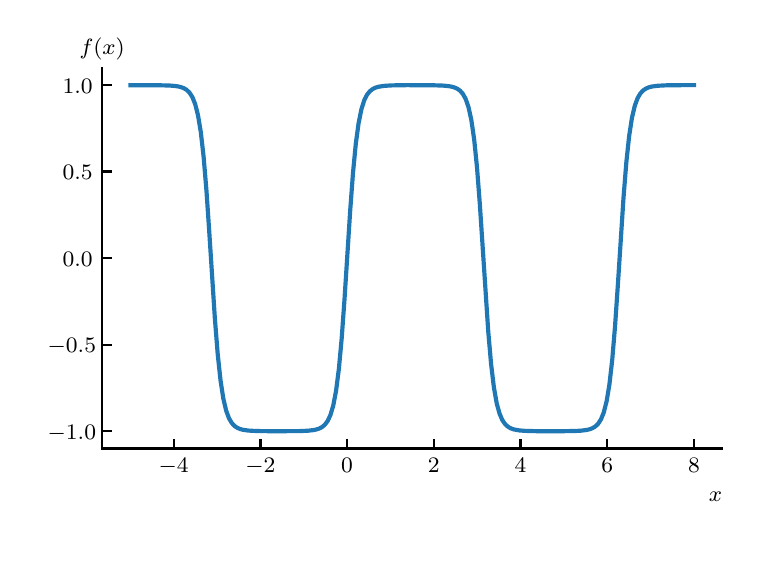
\begin{tikzpicture}%
\node[inner sep=0pt] {%% Creator: Matplotlib, PGF backend
%%
%% To include the figure in your LaTeX document, write
%%   \input{<filename>.pgf}
%%
%% Make sure the required packages are loaded in your preamble
%%   \usepackage{pgf}
%%
%% Also ensure that all the required font packages are loaded; for instance,
%% the lmodern package is sometimes necessary when using math font.
%%   \usepackage{lmodern}
%%
%% Figures using additional raster images can only be included by \input if
%% they are in the same directory as the main LaTeX file. For loading figures
%% from other directories you can use the `import` package
%%   \usepackage{import}
%%
%% and then include the figures with
%%   \import{<path to file>}{<filename>.pgf}
%%
%% Matplotlib used the following preamble
%%   \def\mathdefault#1{#1}
%%   \everymath=\expandafter{\the\everymath\displaystyle}
%%   \RequirePackage[T1]{fontenc}%
%%   \usepackage{newpxmath} % math font is Palatino compatible
%%   \let\Bbbk\relax % so it doesn't clash with amssymb
%%   \usepackage[no-math]{fontspec}
%%   \setmainfont{Palatino}
%%   \setmonofont{Latin Modern Mono}[%
%%   Scale=1.05, % a touch smaller than MatchLowercase
%%   BoldFont=*,
%%   BoldFeatures={FakeBold=2}
%%   ]
%%   \setsansfont{Helvetica}
%%   \renewcommand{\mathdefault}[1][]{}
%%   \usepackage{fontspec}
%%   \setmainfont{Palatino.ttc}[Path=\detokenize{/System/Library/Fonts/}]
%%   \setsansfont{DejaVuSans.ttf}[Path=\detokenize{/Users/ricopicone/anaconda3/envs/engcom/lib/python3.11/site-packages/matplotlib/mpl-data/fonts/ttf/}]
%%   \setmonofont{DejaVuSansMono.ttf}[Path=\detokenize{/Users/ricopicone/anaconda3/envs/engcom/lib/python3.11/site-packages/matplotlib/mpl-data/fonts/ttf/}]
%%   \makeatletter\@ifpackageloaded{underscore}{}{\usepackage[strings]{underscore}}\makeatother
%%
\begingroup%
\makeatletter%
\begin{pgfpicture}%
\pgfpathrectangle{\pgfpointorigin}{\pgfqpoint{3.572444in}{2.531446in}}%
\pgfusepath{use as bounding box, clip}%
\begin{pgfscope}%
\pgfsetbuttcap%
\pgfsetmiterjoin%
\definecolor{currentfill}{rgb}{1.000000,1.000000,1.000000}%
\pgfsetfillcolor{currentfill}%
\pgfsetlinewidth{0.000000pt}%
\definecolor{currentstroke}{rgb}{1.000000,1.000000,1.000000}%
\pgfsetstrokecolor{currentstroke}%
\pgfsetdash{}{0pt}%
\pgfpathmoveto{\pgfqpoint{0.000000in}{0.000000in}}%
\pgfpathlineto{\pgfqpoint{3.572444in}{0.000000in}}%
\pgfpathlineto{\pgfqpoint{3.572444in}{2.531446in}}%
\pgfpathlineto{\pgfqpoint{0.000000in}{2.531446in}}%
\pgfpathlineto{\pgfqpoint{0.000000in}{0.000000in}}%
\pgfpathclose%
\pgfusepath{fill}%
\end{pgfscope}%
\begin{pgfscope}%
\pgfsetbuttcap%
\pgfsetmiterjoin%
\definecolor{currentfill}{rgb}{1.000000,1.000000,1.000000}%
\pgfsetfillcolor{currentfill}%
\pgfsetlinewidth{0.000000pt}%
\definecolor{currentstroke}{rgb}{0.000000,0.000000,0.000000}%
\pgfsetstrokecolor{currentstroke}%
\pgfsetstrokeopacity{0.000000}%
\pgfsetdash{}{0pt}%
\pgfpathmoveto{\pgfqpoint{0.372444in}{0.427040in}}%
\pgfpathlineto{\pgfqpoint{3.472444in}{0.427040in}}%
\pgfpathlineto{\pgfqpoint{3.472444in}{2.330625in}}%
\pgfpathlineto{\pgfqpoint{0.372444in}{2.330625in}}%
\pgfpathlineto{\pgfqpoint{0.372444in}{0.427040in}}%
\pgfpathclose%
\pgfusepath{fill}%
\end{pgfscope}%
\begin{pgfscope}%
\pgfsetbuttcap%
\pgfsetroundjoin%
\definecolor{currentfill}{rgb}{0.000000,0.000000,0.000000}%
\pgfsetfillcolor{currentfill}%
\pgfsetlinewidth{0.803000pt}%
\definecolor{currentstroke}{rgb}{0.000000,0.000000,0.000000}%
\pgfsetstrokecolor{currentstroke}%
\pgfsetdash{}{0pt}%
\pgfsys@defobject{currentmarker}{\pgfqpoint{0.000000in}{0.000000in}}{\pgfqpoint{0.000000in}{0.048611in}}{%
\pgfpathmoveto{\pgfqpoint{0.000000in}{0.000000in}}%
\pgfpathlineto{\pgfqpoint{0.000000in}{0.048611in}}%
\pgfusepath{stroke,fill}%
}%
\begin{pgfscope}%
\pgfsys@transformshift{0.730136in}{0.427040in}%
\pgfsys@useobject{currentmarker}{}%
\end{pgfscope}%
\end{pgfscope}%
\begin{pgfscope}%
\definecolor{textcolor}{rgb}{0.000000,0.000000,0.000000}%
\pgfsetstrokecolor{textcolor}%
\pgfsetfillcolor{textcolor}%
\pgftext[x=0.730136in,y=0.378429in,,top]{\color{textcolor}{\rmfamily\fontsize{8.000000}{9.600000}\selectfont\catcode`\^=\active\def^{\ifmmode\sp\else\^{}\fi}\catcode`\%=\active\def%{\%}$\mathdefault{\ensuremath{-}4}$}}%
\end{pgfscope}%
\begin{pgfscope}%
\pgfsetbuttcap%
\pgfsetroundjoin%
\definecolor{currentfill}{rgb}{0.000000,0.000000,0.000000}%
\pgfsetfillcolor{currentfill}%
\pgfsetlinewidth{0.803000pt}%
\definecolor{currentstroke}{rgb}{0.000000,0.000000,0.000000}%
\pgfsetstrokecolor{currentstroke}%
\pgfsetdash{}{0pt}%
\pgfsys@defobject{currentmarker}{\pgfqpoint{0.000000in}{0.000000in}}{\pgfqpoint{0.000000in}{0.048611in}}{%
\pgfpathmoveto{\pgfqpoint{0.000000in}{0.000000in}}%
\pgfpathlineto{\pgfqpoint{0.000000in}{0.048611in}}%
\pgfusepath{stroke,fill}%
}%
\begin{pgfscope}%
\pgfsys@transformshift{1.163703in}{0.427040in}%
\pgfsys@useobject{currentmarker}{}%
\end{pgfscope}%
\end{pgfscope}%
\begin{pgfscope}%
\definecolor{textcolor}{rgb}{0.000000,0.000000,0.000000}%
\pgfsetstrokecolor{textcolor}%
\pgfsetfillcolor{textcolor}%
\pgftext[x=1.163703in,y=0.378429in,,top]{\color{textcolor}{\rmfamily\fontsize{8.000000}{9.600000}\selectfont\catcode`\^=\active\def^{\ifmmode\sp\else\^{}\fi}\catcode`\%=\active\def%{\%}$\mathdefault{\ensuremath{-}2}$}}%
\end{pgfscope}%
\begin{pgfscope}%
\pgfsetbuttcap%
\pgfsetroundjoin%
\definecolor{currentfill}{rgb}{0.000000,0.000000,0.000000}%
\pgfsetfillcolor{currentfill}%
\pgfsetlinewidth{0.803000pt}%
\definecolor{currentstroke}{rgb}{0.000000,0.000000,0.000000}%
\pgfsetstrokecolor{currentstroke}%
\pgfsetdash{}{0pt}%
\pgfsys@defobject{currentmarker}{\pgfqpoint{0.000000in}{0.000000in}}{\pgfqpoint{0.000000in}{0.048611in}}{%
\pgfpathmoveto{\pgfqpoint{0.000000in}{0.000000in}}%
\pgfpathlineto{\pgfqpoint{0.000000in}{0.048611in}}%
\pgfusepath{stroke,fill}%
}%
\begin{pgfscope}%
\pgfsys@transformshift{1.597269in}{0.427040in}%
\pgfsys@useobject{currentmarker}{}%
\end{pgfscope}%
\end{pgfscope}%
\begin{pgfscope}%
\definecolor{textcolor}{rgb}{0.000000,0.000000,0.000000}%
\pgfsetstrokecolor{textcolor}%
\pgfsetfillcolor{textcolor}%
\pgftext[x=1.597269in,y=0.378429in,,top]{\color{textcolor}{\rmfamily\fontsize{8.000000}{9.600000}\selectfont\catcode`\^=\active\def^{\ifmmode\sp\else\^{}\fi}\catcode`\%=\active\def%{\%}$\mathdefault{0}$}}%
\end{pgfscope}%
\begin{pgfscope}%
\pgfsetbuttcap%
\pgfsetroundjoin%
\definecolor{currentfill}{rgb}{0.000000,0.000000,0.000000}%
\pgfsetfillcolor{currentfill}%
\pgfsetlinewidth{0.803000pt}%
\definecolor{currentstroke}{rgb}{0.000000,0.000000,0.000000}%
\pgfsetstrokecolor{currentstroke}%
\pgfsetdash{}{0pt}%
\pgfsys@defobject{currentmarker}{\pgfqpoint{0.000000in}{0.000000in}}{\pgfqpoint{0.000000in}{0.048611in}}{%
\pgfpathmoveto{\pgfqpoint{0.000000in}{0.000000in}}%
\pgfpathlineto{\pgfqpoint{0.000000in}{0.048611in}}%
\pgfusepath{stroke,fill}%
}%
\begin{pgfscope}%
\pgfsys@transformshift{2.030836in}{0.427040in}%
\pgfsys@useobject{currentmarker}{}%
\end{pgfscope}%
\end{pgfscope}%
\begin{pgfscope}%
\definecolor{textcolor}{rgb}{0.000000,0.000000,0.000000}%
\pgfsetstrokecolor{textcolor}%
\pgfsetfillcolor{textcolor}%
\pgftext[x=2.030836in,y=0.378429in,,top]{\color{textcolor}{\rmfamily\fontsize{8.000000}{9.600000}\selectfont\catcode`\^=\active\def^{\ifmmode\sp\else\^{}\fi}\catcode`\%=\active\def%{\%}$\mathdefault{2}$}}%
\end{pgfscope}%
\begin{pgfscope}%
\pgfsetbuttcap%
\pgfsetroundjoin%
\definecolor{currentfill}{rgb}{0.000000,0.000000,0.000000}%
\pgfsetfillcolor{currentfill}%
\pgfsetlinewidth{0.803000pt}%
\definecolor{currentstroke}{rgb}{0.000000,0.000000,0.000000}%
\pgfsetstrokecolor{currentstroke}%
\pgfsetdash{}{0pt}%
\pgfsys@defobject{currentmarker}{\pgfqpoint{0.000000in}{0.000000in}}{\pgfqpoint{0.000000in}{0.048611in}}{%
\pgfpathmoveto{\pgfqpoint{0.000000in}{0.000000in}}%
\pgfpathlineto{\pgfqpoint{0.000000in}{0.048611in}}%
\pgfusepath{stroke,fill}%
}%
\begin{pgfscope}%
\pgfsys@transformshift{2.464402in}{0.427040in}%
\pgfsys@useobject{currentmarker}{}%
\end{pgfscope}%
\end{pgfscope}%
\begin{pgfscope}%
\definecolor{textcolor}{rgb}{0.000000,0.000000,0.000000}%
\pgfsetstrokecolor{textcolor}%
\pgfsetfillcolor{textcolor}%
\pgftext[x=2.464402in,y=0.378429in,,top]{\color{textcolor}{\rmfamily\fontsize{8.000000}{9.600000}\selectfont\catcode`\^=\active\def^{\ifmmode\sp\else\^{}\fi}\catcode`\%=\active\def%{\%}$\mathdefault{4}$}}%
\end{pgfscope}%
\begin{pgfscope}%
\pgfsetbuttcap%
\pgfsetroundjoin%
\definecolor{currentfill}{rgb}{0.000000,0.000000,0.000000}%
\pgfsetfillcolor{currentfill}%
\pgfsetlinewidth{0.803000pt}%
\definecolor{currentstroke}{rgb}{0.000000,0.000000,0.000000}%
\pgfsetstrokecolor{currentstroke}%
\pgfsetdash{}{0pt}%
\pgfsys@defobject{currentmarker}{\pgfqpoint{0.000000in}{0.000000in}}{\pgfqpoint{0.000000in}{0.048611in}}{%
\pgfpathmoveto{\pgfqpoint{0.000000in}{0.000000in}}%
\pgfpathlineto{\pgfqpoint{0.000000in}{0.048611in}}%
\pgfusepath{stroke,fill}%
}%
\begin{pgfscope}%
\pgfsys@transformshift{2.897969in}{0.427040in}%
\pgfsys@useobject{currentmarker}{}%
\end{pgfscope}%
\end{pgfscope}%
\begin{pgfscope}%
\definecolor{textcolor}{rgb}{0.000000,0.000000,0.000000}%
\pgfsetstrokecolor{textcolor}%
\pgfsetfillcolor{textcolor}%
\pgftext[x=2.897969in,y=0.378429in,,top]{\color{textcolor}{\rmfamily\fontsize{8.000000}{9.600000}\selectfont\catcode`\^=\active\def^{\ifmmode\sp\else\^{}\fi}\catcode`\%=\active\def%{\%}$\mathdefault{6}$}}%
\end{pgfscope}%
\begin{pgfscope}%
\pgfsetbuttcap%
\pgfsetroundjoin%
\definecolor{currentfill}{rgb}{0.000000,0.000000,0.000000}%
\pgfsetfillcolor{currentfill}%
\pgfsetlinewidth{0.803000pt}%
\definecolor{currentstroke}{rgb}{0.000000,0.000000,0.000000}%
\pgfsetstrokecolor{currentstroke}%
\pgfsetdash{}{0pt}%
\pgfsys@defobject{currentmarker}{\pgfqpoint{0.000000in}{0.000000in}}{\pgfqpoint{0.000000in}{0.048611in}}{%
\pgfpathmoveto{\pgfqpoint{0.000000in}{0.000000in}}%
\pgfpathlineto{\pgfqpoint{0.000000in}{0.048611in}}%
\pgfusepath{stroke,fill}%
}%
\begin{pgfscope}%
\pgfsys@transformshift{3.331535in}{0.427040in}%
\pgfsys@useobject{currentmarker}{}%
\end{pgfscope}%
\end{pgfscope}%
\begin{pgfscope}%
\definecolor{textcolor}{rgb}{0.000000,0.000000,0.000000}%
\pgfsetstrokecolor{textcolor}%
\pgfsetfillcolor{textcolor}%
\pgftext[x=3.331535in,y=0.378429in,,top]{\color{textcolor}{\rmfamily\fontsize{8.000000}{9.600000}\selectfont\catcode`\^=\active\def^{\ifmmode\sp\else\^{}\fi}\catcode`\%=\active\def%{\%}$\mathdefault{8}$}}%
\end{pgfscope}%
\begin{pgfscope}%
\definecolor{textcolor}{rgb}{0.000000,0.000000,0.000000}%
\pgfsetstrokecolor{textcolor}%
\pgfsetfillcolor{textcolor}%
\pgftext[x=3.472444in,y=0.211437in,right,top]{\color{textcolor}{\rmfamily\fontsize{8.000000}{9.600000}\selectfont\catcode`\^=\active\def^{\ifmmode\sp\else\^{}\fi}\catcode`\%=\active\def%{\%}$x$}}%
\end{pgfscope}%
\begin{pgfscope}%
\pgfsetbuttcap%
\pgfsetroundjoin%
\definecolor{currentfill}{rgb}{0.000000,0.000000,0.000000}%
\pgfsetfillcolor{currentfill}%
\pgfsetlinewidth{0.803000pt}%
\definecolor{currentstroke}{rgb}{0.000000,0.000000,0.000000}%
\pgfsetstrokecolor{currentstroke}%
\pgfsetdash{}{0pt}%
\pgfsys@defobject{currentmarker}{\pgfqpoint{0.000000in}{0.000000in}}{\pgfqpoint{0.048611in}{0.000000in}}{%
\pgfpathmoveto{\pgfqpoint{0.000000in}{0.000000in}}%
\pgfpathlineto{\pgfqpoint{0.048611in}{0.000000in}}%
\pgfusepath{stroke,fill}%
}%
\begin{pgfscope}%
\pgfsys@transformshift{0.372444in}{0.512985in}%
\pgfsys@useobject{currentmarker}{}%
\end{pgfscope}%
\end{pgfscope}%
\begin{pgfscope}%
\definecolor{textcolor}{rgb}{0.000000,0.000000,0.000000}%
\pgfsetstrokecolor{textcolor}%
\pgfsetfillcolor{textcolor}%
\pgftext[x=0.100000in, y=0.472566in, left, base]{\color{textcolor}{\rmfamily\fontsize{8.000000}{9.600000}\selectfont\catcode`\^=\active\def^{\ifmmode\sp\else\^{}\fi}\catcode`\%=\active\def%{\%}$\mathdefault{\ensuremath{-}1.0}$}}%
\end{pgfscope}%
\begin{pgfscope}%
\pgfsetbuttcap%
\pgfsetroundjoin%
\definecolor{currentfill}{rgb}{0.000000,0.000000,0.000000}%
\pgfsetfillcolor{currentfill}%
\pgfsetlinewidth{0.803000pt}%
\definecolor{currentstroke}{rgb}{0.000000,0.000000,0.000000}%
\pgfsetstrokecolor{currentstroke}%
\pgfsetdash{}{0pt}%
\pgfsys@defobject{currentmarker}{\pgfqpoint{0.000000in}{0.000000in}}{\pgfqpoint{0.048611in}{0.000000in}}{%
\pgfpathmoveto{\pgfqpoint{0.000000in}{0.000000in}}%
\pgfpathlineto{\pgfqpoint{0.048611in}{0.000000in}}%
\pgfusepath{stroke,fill}%
}%
\begin{pgfscope}%
\pgfsys@transformshift{0.372444in}{0.945909in}%
\pgfsys@useobject{currentmarker}{}%
\end{pgfscope}%
\end{pgfscope}%
\begin{pgfscope}%
\definecolor{textcolor}{rgb}{0.000000,0.000000,0.000000}%
\pgfsetstrokecolor{textcolor}%
\pgfsetfillcolor{textcolor}%
\pgftext[x=0.100000in, y=0.905490in, left, base]{\color{textcolor}{\rmfamily\fontsize{8.000000}{9.600000}\selectfont\catcode`\^=\active\def^{\ifmmode\sp\else\^{}\fi}\catcode`\%=\active\def%{\%}$\mathdefault{\ensuremath{-}0.5}$}}%
\end{pgfscope}%
\begin{pgfscope}%
\pgfsetbuttcap%
\pgfsetroundjoin%
\definecolor{currentfill}{rgb}{0.000000,0.000000,0.000000}%
\pgfsetfillcolor{currentfill}%
\pgfsetlinewidth{0.803000pt}%
\definecolor{currentstroke}{rgb}{0.000000,0.000000,0.000000}%
\pgfsetstrokecolor{currentstroke}%
\pgfsetdash{}{0pt}%
\pgfsys@defobject{currentmarker}{\pgfqpoint{0.000000in}{0.000000in}}{\pgfqpoint{0.048611in}{0.000000in}}{%
\pgfpathmoveto{\pgfqpoint{0.000000in}{0.000000in}}%
\pgfpathlineto{\pgfqpoint{0.048611in}{0.000000in}}%
\pgfusepath{stroke,fill}%
}%
\begin{pgfscope}%
\pgfsys@transformshift{0.372444in}{1.378832in}%
\pgfsys@useobject{currentmarker}{}%
\end{pgfscope}%
\end{pgfscope}%
\begin{pgfscope}%
\definecolor{textcolor}{rgb}{0.000000,0.000000,0.000000}%
\pgfsetstrokecolor{textcolor}%
\pgfsetfillcolor{textcolor}%
\pgftext[x=0.174333in, y=1.338413in, left, base]{\color{textcolor}{\rmfamily\fontsize{8.000000}{9.600000}\selectfont\catcode`\^=\active\def^{\ifmmode\sp\else\^{}\fi}\catcode`\%=\active\def%{\%}$\mathdefault{0.0}$}}%
\end{pgfscope}%
\begin{pgfscope}%
\pgfsetbuttcap%
\pgfsetroundjoin%
\definecolor{currentfill}{rgb}{0.000000,0.000000,0.000000}%
\pgfsetfillcolor{currentfill}%
\pgfsetlinewidth{0.803000pt}%
\definecolor{currentstroke}{rgb}{0.000000,0.000000,0.000000}%
\pgfsetstrokecolor{currentstroke}%
\pgfsetdash{}{0pt}%
\pgfsys@defobject{currentmarker}{\pgfqpoint{0.000000in}{0.000000in}}{\pgfqpoint{0.048611in}{0.000000in}}{%
\pgfpathmoveto{\pgfqpoint{0.000000in}{0.000000in}}%
\pgfpathlineto{\pgfqpoint{0.048611in}{0.000000in}}%
\pgfusepath{stroke,fill}%
}%
\begin{pgfscope}%
\pgfsys@transformshift{0.372444in}{1.811755in}%
\pgfsys@useobject{currentmarker}{}%
\end{pgfscope}%
\end{pgfscope}%
\begin{pgfscope}%
\definecolor{textcolor}{rgb}{0.000000,0.000000,0.000000}%
\pgfsetstrokecolor{textcolor}%
\pgfsetfillcolor{textcolor}%
\pgftext[x=0.174333in, y=1.771337in, left, base]{\color{textcolor}{\rmfamily\fontsize{8.000000}{9.600000}\selectfont\catcode`\^=\active\def^{\ifmmode\sp\else\^{}\fi}\catcode`\%=\active\def%{\%}$\mathdefault{0.5}$}}%
\end{pgfscope}%
\begin{pgfscope}%
\pgfsetbuttcap%
\pgfsetroundjoin%
\definecolor{currentfill}{rgb}{0.000000,0.000000,0.000000}%
\pgfsetfillcolor{currentfill}%
\pgfsetlinewidth{0.803000pt}%
\definecolor{currentstroke}{rgb}{0.000000,0.000000,0.000000}%
\pgfsetstrokecolor{currentstroke}%
\pgfsetdash{}{0pt}%
\pgfsys@defobject{currentmarker}{\pgfqpoint{0.000000in}{0.000000in}}{\pgfqpoint{0.048611in}{0.000000in}}{%
\pgfpathmoveto{\pgfqpoint{0.000000in}{0.000000in}}%
\pgfpathlineto{\pgfqpoint{0.048611in}{0.000000in}}%
\pgfusepath{stroke,fill}%
}%
\begin{pgfscope}%
\pgfsys@transformshift{0.372444in}{2.244679in}%
\pgfsys@useobject{currentmarker}{}%
\end{pgfscope}%
\end{pgfscope}%
\begin{pgfscope}%
\definecolor{textcolor}{rgb}{0.000000,0.000000,0.000000}%
\pgfsetstrokecolor{textcolor}%
\pgfsetfillcolor{textcolor}%
\pgftext[x=0.174333in, y=2.204260in, left, base]{\color{textcolor}{\rmfamily\fontsize{8.000000}{9.600000}\selectfont\catcode`\^=\active\def^{\ifmmode\sp\else\^{}\fi}\catcode`\%=\active\def%{\%}$\mathdefault{1.0}$}}%
\end{pgfscope}%
\begin{pgfscope}%
\definecolor{textcolor}{rgb}{0.000000,0.000000,0.000000}%
\pgfsetstrokecolor{textcolor}%
\pgfsetfillcolor{textcolor}%
\pgftext[x=0.372444in,y=2.368696in,,bottom]{\color{textcolor}{\rmfamily\fontsize{8.000000}{9.600000}\selectfont\catcode`\^=\active\def^{\ifmmode\sp\else\^{}\fi}\catcode`\%=\active\def%{\%}$f(x)$}}%
\end{pgfscope}%
\begin{pgfscope}%
\pgfpathrectangle{\pgfqpoint{0.372444in}{0.427040in}}{\pgfqpoint{3.100000in}{1.903585in}}%
\pgfusepath{clip}%
\pgfsetrectcap%
\pgfsetroundjoin%
\pgfsetlinewidth{1.505625pt}%
\definecolor{currentstroke}{rgb}{0.121569,0.466667,0.705882}%
\pgfsetstrokecolor{currentstroke}%
\pgfsetdash{}{0pt}%
\pgfpathmoveto{\pgfqpoint{0.513353in}{2.243872in}}%
\pgfpathlineto{\pgfqpoint{0.640171in}{2.243854in}}%
\pgfpathlineto{\pgfqpoint{0.710626in}{2.242079in}}%
\pgfpathlineto{\pgfqpoint{0.738808in}{2.239659in}}%
\pgfpathlineto{\pgfqpoint{0.752899in}{2.237439in}}%
\pgfpathlineto{\pgfqpoint{0.766990in}{2.234001in}}%
\pgfpathlineto{\pgfqpoint{0.781081in}{2.228607in}}%
\pgfpathlineto{\pgfqpoint{0.795171in}{2.220052in}}%
\pgfpathlineto{\pgfqpoint{0.809262in}{2.206379in}}%
\pgfpathlineto{\pgfqpoint{0.823353in}{2.184455in}}%
\pgfpathlineto{\pgfqpoint{0.837444in}{2.149421in}}%
\pgfpathlineto{\pgfqpoint{0.851535in}{2.094181in}}%
\pgfpathlineto{\pgfqpoint{0.865626in}{2.009460in}}%
\pgfpathlineto{\pgfqpoint{0.879717in}{1.885591in}}%
\pgfpathlineto{\pgfqpoint{0.893808in}{1.717314in}}%
\pgfpathlineto{\pgfqpoint{0.907899in}{1.510783in}}%
\pgfpathlineto{\pgfqpoint{0.936081in}{1.075471in}}%
\pgfpathlineto{\pgfqpoint{0.950171in}{0.899345in}}%
\pgfpathlineto{\pgfqpoint{0.964262in}{0.767557in}}%
\pgfpathlineto{\pgfqpoint{0.978353in}{0.676394in}}%
\pgfpathlineto{\pgfqpoint{0.992444in}{0.616535in}}%
\pgfpathlineto{\pgfqpoint{1.006535in}{0.578427in}}%
\pgfpathlineto{\pgfqpoint{1.020626in}{0.554541in}}%
\pgfpathlineto{\pgfqpoint{1.034717in}{0.539644in}}%
\pgfpathlineto{\pgfqpoint{1.048808in}{0.530332in}}%
\pgfpathlineto{\pgfqpoint{1.062899in}{0.524471in}}%
\pgfpathlineto{\pgfqpoint{1.076990in}{0.520743in}}%
\pgfpathlineto{\pgfqpoint{1.105171in}{0.516773in}}%
\pgfpathlineto{\pgfqpoint{1.147444in}{0.514556in}}%
\pgfpathlineto{\pgfqpoint{1.231990in}{0.513597in}}%
\pgfpathlineto{\pgfqpoint{1.358808in}{0.514371in}}%
\pgfpathlineto{\pgfqpoint{1.401081in}{0.516187in}}%
\pgfpathlineto{\pgfqpoint{1.429262in}{0.519380in}}%
\pgfpathlineto{\pgfqpoint{1.443353in}{0.522348in}}%
\pgfpathlineto{\pgfqpoint{1.457444in}{0.526987in}}%
\pgfpathlineto{\pgfqpoint{1.471535in}{0.534319in}}%
\pgfpathlineto{\pgfqpoint{1.485626in}{0.546012in}}%
\pgfpathlineto{\pgfqpoint{1.499717in}{0.564754in}}%
\pgfpathlineto{\pgfqpoint{1.513808in}{0.594763in}}%
\pgfpathlineto{\pgfqpoint{1.527899in}{0.642355in}}%
\pgfpathlineto{\pgfqpoint{1.541990in}{0.716164in}}%
\pgfpathlineto{\pgfqpoint{1.556081in}{0.826092in}}%
\pgfpathlineto{\pgfqpoint{1.570171in}{0.979596in}}%
\pgfpathlineto{\pgfqpoint{1.584262in}{1.175047in}}%
\pgfpathlineto{\pgfqpoint{1.612444in}{1.614943in}}%
\pgfpathlineto{\pgfqpoint{1.626535in}{1.804609in}}%
\pgfpathlineto{\pgfqpoint{1.640626in}{1.951201in}}%
\pgfpathlineto{\pgfqpoint{1.654717in}{2.054960in}}%
\pgfpathlineto{\pgfqpoint{1.668808in}{2.124096in}}%
\pgfpathlineto{\pgfqpoint{1.682899in}{2.168477in}}%
\pgfpathlineto{\pgfqpoint{1.696990in}{2.196400in}}%
\pgfpathlineto{\pgfqpoint{1.711081in}{2.213828in}}%
\pgfpathlineto{\pgfqpoint{1.725171in}{2.224706in}}%
\pgfpathlineto{\pgfqpoint{1.739262in}{2.231535in}}%
\pgfpathlineto{\pgfqpoint{1.753353in}{2.235862in}}%
\pgfpathlineto{\pgfqpoint{1.781535in}{2.240441in}}%
\pgfpathlineto{\pgfqpoint{1.823808in}{2.242969in}}%
\pgfpathlineto{\pgfqpoint{1.894262in}{2.243997in}}%
\pgfpathlineto{\pgfqpoint{2.021081in}{2.243639in}}%
\pgfpathlineto{\pgfqpoint{2.077444in}{2.241797in}}%
\pgfpathlineto{\pgfqpoint{2.105626in}{2.239017in}}%
\pgfpathlineto{\pgfqpoint{2.119717in}{2.236450in}}%
\pgfpathlineto{\pgfqpoint{2.133808in}{2.232456in}}%
\pgfpathlineto{\pgfqpoint{2.147899in}{2.226166in}}%
\pgfpathlineto{\pgfqpoint{2.161990in}{2.216160in}}%
\pgfpathlineto{\pgfqpoint{2.176081in}{2.200140in}}%
\pgfpathlineto{\pgfqpoint{2.190171in}{2.174461in}}%
\pgfpathlineto{\pgfqpoint{2.204262in}{2.133557in}}%
\pgfpathlineto{\pgfqpoint{2.218353in}{2.069538in}}%
\pgfpathlineto{\pgfqpoint{2.232444in}{1.972669in}}%
\pgfpathlineto{\pgfqpoint{2.246535in}{1.834063in}}%
\pgfpathlineto{\pgfqpoint{2.260626in}{1.651513in}}%
\pgfpathlineto{\pgfqpoint{2.302899in}{1.011643in}}%
\pgfpathlineto{\pgfqpoint{2.316990in}{0.850161in}}%
\pgfpathlineto{\pgfqpoint{2.331081in}{0.732845in}}%
\pgfpathlineto{\pgfqpoint{2.345171in}{0.653318in}}%
\pgfpathlineto{\pgfqpoint{2.359262in}{0.601744in}}%
\pgfpathlineto{\pgfqpoint{2.373353in}{0.569129in}}%
\pgfpathlineto{\pgfqpoint{2.387444in}{0.548740in}}%
\pgfpathlineto{\pgfqpoint{2.401535in}{0.536023in}}%
\pgfpathlineto{\pgfqpoint{2.415626in}{0.528059in}}%
\pgfpathlineto{\pgfqpoint{2.429717in}{0.523030in}}%
\pgfpathlineto{\pgfqpoint{2.457899in}{0.517741in}}%
\pgfpathlineto{\pgfqpoint{2.486081in}{0.515468in}}%
\pgfpathlineto{\pgfqpoint{2.542444in}{0.513935in}}%
\pgfpathlineto{\pgfqpoint{2.669262in}{0.513706in}}%
\pgfpathlineto{\pgfqpoint{2.739717in}{0.514935in}}%
\pgfpathlineto{\pgfqpoint{2.767899in}{0.516556in}}%
\pgfpathlineto{\pgfqpoint{2.796081in}{0.520235in}}%
\pgfpathlineto{\pgfqpoint{2.810171in}{0.523678in}}%
\pgfpathlineto{\pgfqpoint{2.824262in}{0.529080in}}%
\pgfpathlineto{\pgfqpoint{2.838353in}{0.537649in}}%
\pgfpathlineto{\pgfqpoint{2.852444in}{0.551344in}}%
\pgfpathlineto{\pgfqpoint{2.866535in}{0.573304in}}%
\pgfpathlineto{\pgfqpoint{2.880626in}{0.608393in}}%
\pgfpathlineto{\pgfqpoint{2.894717in}{0.663717in}}%
\pgfpathlineto{\pgfqpoint{2.908808in}{0.748556in}}%
\pgfpathlineto{\pgfqpoint{2.922899in}{0.872572in}}%
\pgfpathlineto{\pgfqpoint{2.936990in}{1.040998in}}%
\pgfpathlineto{\pgfqpoint{2.951081in}{1.247632in}}%
\pgfpathlineto{\pgfqpoint{2.979262in}{1.682865in}}%
\pgfpathlineto{\pgfqpoint{2.993353in}{1.858845in}}%
\pgfpathlineto{\pgfqpoint{3.007444in}{1.990483in}}%
\pgfpathlineto{\pgfqpoint{3.021535in}{2.081522in}}%
\pgfpathlineto{\pgfqpoint{3.035626in}{2.141292in}}%
\pgfpathlineto{\pgfqpoint{3.049717in}{2.179340in}}%
\pgfpathlineto{\pgfqpoint{3.063808in}{2.203187in}}%
\pgfpathlineto{\pgfqpoint{3.077899in}{2.218060in}}%
\pgfpathlineto{\pgfqpoint{3.091990in}{2.227357in}}%
\pgfpathlineto{\pgfqpoint{3.106081in}{2.233209in}}%
\pgfpathlineto{\pgfqpoint{3.120171in}{2.236932in}}%
\pgfpathlineto{\pgfqpoint{3.148353in}{2.240895in}}%
\pgfpathlineto{\pgfqpoint{3.190626in}{2.243110in}}%
\pgfpathlineto{\pgfqpoint{3.275171in}{2.244067in}}%
\pgfpathlineto{\pgfqpoint{3.331535in}{2.244047in}}%
\pgfpathlineto{\pgfqpoint{3.331535in}{2.244047in}}%
\pgfusepath{stroke}%
\end{pgfscope}%
\begin{pgfscope}%
\pgfsetrectcap%
\pgfsetmiterjoin%
\pgfsetlinewidth{0.803000pt}%
\definecolor{currentstroke}{rgb}{0.000000,0.000000,0.000000}%
\pgfsetstrokecolor{currentstroke}%
\pgfsetdash{}{0pt}%
\pgfpathmoveto{\pgfqpoint{0.372444in}{0.427040in}}%
\pgfpathlineto{\pgfqpoint{0.372444in}{2.330625in}}%
\pgfusepath{stroke}%
\end{pgfscope}%
\begin{pgfscope}%
\pgfsetrectcap%
\pgfsetmiterjoin%
\pgfsetlinewidth{0.803000pt}%
\definecolor{currentstroke}{rgb}{0.000000,0.000000,0.000000}%
\pgfsetstrokecolor{currentstroke}%
\pgfsetdash{}{0pt}%
\pgfpathmoveto{\pgfqpoint{0.372444in}{0.427040in}}%
\pgfpathlineto{\pgfqpoint{3.472444in}{0.427040in}}%
\pgfusepath{stroke}%
\end{pgfscope}%
\end{pgfpicture}%
\makeatother%
\endgroup%
};%
\end{tikzpicture}%
\caption{}
\label{fig:publishing_with_makefile-figure-0}
\end{figure}

\phantomsection\label{1175bdd1}
Plot $g(x)$:

\phantomsection\label{aeb25cc0}
\nointerlineskip\nointerlineskip\begin{minted}[autogobble,samepage]{python}
fig, ax = plt.subplots()
plotter(fig, fun=g, limits=(0, 100), labels=("$x$", "$g(x)$"))
\end{minted}

\phantomsection\label{e9a16f44}
\gdef\graphicslist{}%
\begin{figure}[htbp]
\centering
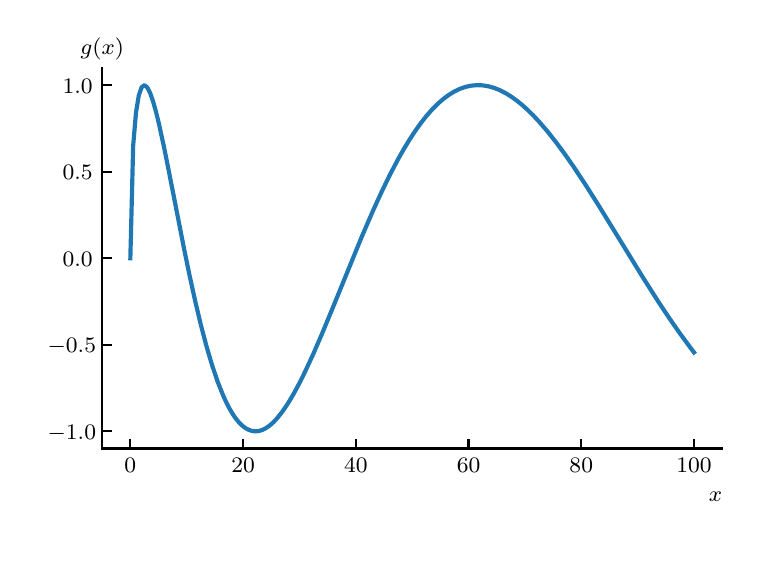
\begin{tikzpicture}%
\node[inner sep=0pt] {%% Creator: Matplotlib, PGF backend
%%
%% To include the figure in your LaTeX document, write
%%   \input{<filename>.pgf}
%%
%% Make sure the required packages are loaded in your preamble
%%   \usepackage{pgf}
%%
%% Also ensure that all the required font packages are loaded; for instance,
%% the lmodern package is sometimes necessary when using math font.
%%   \usepackage{lmodern}
%%
%% Figures using additional raster images can only be included by \input if
%% they are in the same directory as the main LaTeX file. For loading figures
%% from other directories you can use the `import` package
%%   \usepackage{import}
%%
%% and then include the figures with
%%   \import{<path to file>}{<filename>.pgf}
%%
%% Matplotlib used the following preamble
%%   \def\mathdefault#1{#1}
%%   \everymath=\expandafter{\the\everymath\displaystyle}
%%   \RequirePackage[T1]{fontenc}%
%%   \usepackage{newpxmath} % math font is Palatino compatible
%%   \let\Bbbk\relax % so it doesn't clash with amssymb
%%   \usepackage[no-math]{fontspec}
%%   \setmainfont{Palatino}
%%   \setmonofont{Latin Modern Mono}[%
%%   Scale=1.05, % a touch smaller than MatchLowercase
%%   BoldFont=*,
%%   BoldFeatures={FakeBold=2}
%%   ]
%%   \setsansfont{Helvetica}
%%   \renewcommand{\mathdefault}[1][]{}
%%   \usepackage{fontspec}
%%   \setmainfont{Palatino.ttc}[Path=\detokenize{/System/Library/Fonts/}]
%%   \setsansfont{DejaVuSans.ttf}[Path=\detokenize{/Users/ricopicone/anaconda3/envs/engcom/lib/python3.11/site-packages/matplotlib/mpl-data/fonts/ttf/}]
%%   \setmonofont{DejaVuSansMono.ttf}[Path=\detokenize{/Users/ricopicone/anaconda3/envs/engcom/lib/python3.11/site-packages/matplotlib/mpl-data/fonts/ttf/}]
%%   \makeatletter\@ifpackageloaded{underscore}{}{\usepackage[strings]{underscore}}\makeatother
%%
\begingroup%
\makeatletter%
\begin{pgfpicture}%
\pgfpathrectangle{\pgfpointorigin}{\pgfqpoint{3.572444in}{2.531446in}}%
\pgfusepath{use as bounding box, clip}%
\begin{pgfscope}%
\pgfsetbuttcap%
\pgfsetmiterjoin%
\definecolor{currentfill}{rgb}{1.000000,1.000000,1.000000}%
\pgfsetfillcolor{currentfill}%
\pgfsetlinewidth{0.000000pt}%
\definecolor{currentstroke}{rgb}{1.000000,1.000000,1.000000}%
\pgfsetstrokecolor{currentstroke}%
\pgfsetdash{}{0pt}%
\pgfpathmoveto{\pgfqpoint{0.000000in}{0.000000in}}%
\pgfpathlineto{\pgfqpoint{3.572444in}{0.000000in}}%
\pgfpathlineto{\pgfqpoint{3.572444in}{2.531446in}}%
\pgfpathlineto{\pgfqpoint{0.000000in}{2.531446in}}%
\pgfpathlineto{\pgfqpoint{0.000000in}{0.000000in}}%
\pgfpathclose%
\pgfusepath{fill}%
\end{pgfscope}%
\begin{pgfscope}%
\pgfsetbuttcap%
\pgfsetmiterjoin%
\definecolor{currentfill}{rgb}{1.000000,1.000000,1.000000}%
\pgfsetfillcolor{currentfill}%
\pgfsetlinewidth{0.000000pt}%
\definecolor{currentstroke}{rgb}{0.000000,0.000000,0.000000}%
\pgfsetstrokecolor{currentstroke}%
\pgfsetstrokeopacity{0.000000}%
\pgfsetdash{}{0pt}%
\pgfpathmoveto{\pgfqpoint{0.372444in}{0.427040in}}%
\pgfpathlineto{\pgfqpoint{3.472444in}{0.427040in}}%
\pgfpathlineto{\pgfqpoint{3.472444in}{2.330625in}}%
\pgfpathlineto{\pgfqpoint{0.372444in}{2.330625in}}%
\pgfpathlineto{\pgfqpoint{0.372444in}{0.427040in}}%
\pgfpathclose%
\pgfusepath{fill}%
\end{pgfscope}%
\begin{pgfscope}%
\pgfsetbuttcap%
\pgfsetroundjoin%
\definecolor{currentfill}{rgb}{0.000000,0.000000,0.000000}%
\pgfsetfillcolor{currentfill}%
\pgfsetlinewidth{0.803000pt}%
\definecolor{currentstroke}{rgb}{0.000000,0.000000,0.000000}%
\pgfsetstrokecolor{currentstroke}%
\pgfsetdash{}{0pt}%
\pgfsys@defobject{currentmarker}{\pgfqpoint{0.000000in}{0.000000in}}{\pgfqpoint{0.000000in}{0.048611in}}{%
\pgfpathmoveto{\pgfqpoint{0.000000in}{0.000000in}}%
\pgfpathlineto{\pgfqpoint{0.000000in}{0.048611in}}%
\pgfusepath{stroke,fill}%
}%
\begin{pgfscope}%
\pgfsys@transformshift{0.513353in}{0.427040in}%
\pgfsys@useobject{currentmarker}{}%
\end{pgfscope}%
\end{pgfscope}%
\begin{pgfscope}%
\definecolor{textcolor}{rgb}{0.000000,0.000000,0.000000}%
\pgfsetstrokecolor{textcolor}%
\pgfsetfillcolor{textcolor}%
\pgftext[x=0.513353in,y=0.378429in,,top]{\color{textcolor}{\rmfamily\fontsize{8.000000}{9.600000}\selectfont\catcode`\^=\active\def^{\ifmmode\sp\else\^{}\fi}\catcode`\%=\active\def%{\%}$\mathdefault{0}$}}%
\end{pgfscope}%
\begin{pgfscope}%
\pgfsetbuttcap%
\pgfsetroundjoin%
\definecolor{currentfill}{rgb}{0.000000,0.000000,0.000000}%
\pgfsetfillcolor{currentfill}%
\pgfsetlinewidth{0.803000pt}%
\definecolor{currentstroke}{rgb}{0.000000,0.000000,0.000000}%
\pgfsetstrokecolor{currentstroke}%
\pgfsetdash{}{0pt}%
\pgfsys@defobject{currentmarker}{\pgfqpoint{0.000000in}{0.000000in}}{\pgfqpoint{0.000000in}{0.048611in}}{%
\pgfpathmoveto{\pgfqpoint{0.000000in}{0.000000in}}%
\pgfpathlineto{\pgfqpoint{0.000000in}{0.048611in}}%
\pgfusepath{stroke,fill}%
}%
\begin{pgfscope}%
\pgfsys@transformshift{1.076990in}{0.427040in}%
\pgfsys@useobject{currentmarker}{}%
\end{pgfscope}%
\end{pgfscope}%
\begin{pgfscope}%
\definecolor{textcolor}{rgb}{0.000000,0.000000,0.000000}%
\pgfsetstrokecolor{textcolor}%
\pgfsetfillcolor{textcolor}%
\pgftext[x=1.076990in,y=0.378429in,,top]{\color{textcolor}{\rmfamily\fontsize{8.000000}{9.600000}\selectfont\catcode`\^=\active\def^{\ifmmode\sp\else\^{}\fi}\catcode`\%=\active\def%{\%}$\mathdefault{20}$}}%
\end{pgfscope}%
\begin{pgfscope}%
\pgfsetbuttcap%
\pgfsetroundjoin%
\definecolor{currentfill}{rgb}{0.000000,0.000000,0.000000}%
\pgfsetfillcolor{currentfill}%
\pgfsetlinewidth{0.803000pt}%
\definecolor{currentstroke}{rgb}{0.000000,0.000000,0.000000}%
\pgfsetstrokecolor{currentstroke}%
\pgfsetdash{}{0pt}%
\pgfsys@defobject{currentmarker}{\pgfqpoint{0.000000in}{0.000000in}}{\pgfqpoint{0.000000in}{0.048611in}}{%
\pgfpathmoveto{\pgfqpoint{0.000000in}{0.000000in}}%
\pgfpathlineto{\pgfqpoint{0.000000in}{0.048611in}}%
\pgfusepath{stroke,fill}%
}%
\begin{pgfscope}%
\pgfsys@transformshift{1.640626in}{0.427040in}%
\pgfsys@useobject{currentmarker}{}%
\end{pgfscope}%
\end{pgfscope}%
\begin{pgfscope}%
\definecolor{textcolor}{rgb}{0.000000,0.000000,0.000000}%
\pgfsetstrokecolor{textcolor}%
\pgfsetfillcolor{textcolor}%
\pgftext[x=1.640626in,y=0.378429in,,top]{\color{textcolor}{\rmfamily\fontsize{8.000000}{9.600000}\selectfont\catcode`\^=\active\def^{\ifmmode\sp\else\^{}\fi}\catcode`\%=\active\def%{\%}$\mathdefault{40}$}}%
\end{pgfscope}%
\begin{pgfscope}%
\pgfsetbuttcap%
\pgfsetroundjoin%
\definecolor{currentfill}{rgb}{0.000000,0.000000,0.000000}%
\pgfsetfillcolor{currentfill}%
\pgfsetlinewidth{0.803000pt}%
\definecolor{currentstroke}{rgb}{0.000000,0.000000,0.000000}%
\pgfsetstrokecolor{currentstroke}%
\pgfsetdash{}{0pt}%
\pgfsys@defobject{currentmarker}{\pgfqpoint{0.000000in}{0.000000in}}{\pgfqpoint{0.000000in}{0.048611in}}{%
\pgfpathmoveto{\pgfqpoint{0.000000in}{0.000000in}}%
\pgfpathlineto{\pgfqpoint{0.000000in}{0.048611in}}%
\pgfusepath{stroke,fill}%
}%
\begin{pgfscope}%
\pgfsys@transformshift{2.204262in}{0.427040in}%
\pgfsys@useobject{currentmarker}{}%
\end{pgfscope}%
\end{pgfscope}%
\begin{pgfscope}%
\definecolor{textcolor}{rgb}{0.000000,0.000000,0.000000}%
\pgfsetstrokecolor{textcolor}%
\pgfsetfillcolor{textcolor}%
\pgftext[x=2.204262in,y=0.378429in,,top]{\color{textcolor}{\rmfamily\fontsize{8.000000}{9.600000}\selectfont\catcode`\^=\active\def^{\ifmmode\sp\else\^{}\fi}\catcode`\%=\active\def%{\%}$\mathdefault{60}$}}%
\end{pgfscope}%
\begin{pgfscope}%
\pgfsetbuttcap%
\pgfsetroundjoin%
\definecolor{currentfill}{rgb}{0.000000,0.000000,0.000000}%
\pgfsetfillcolor{currentfill}%
\pgfsetlinewidth{0.803000pt}%
\definecolor{currentstroke}{rgb}{0.000000,0.000000,0.000000}%
\pgfsetstrokecolor{currentstroke}%
\pgfsetdash{}{0pt}%
\pgfsys@defobject{currentmarker}{\pgfqpoint{0.000000in}{0.000000in}}{\pgfqpoint{0.000000in}{0.048611in}}{%
\pgfpathmoveto{\pgfqpoint{0.000000in}{0.000000in}}%
\pgfpathlineto{\pgfqpoint{0.000000in}{0.048611in}}%
\pgfusepath{stroke,fill}%
}%
\begin{pgfscope}%
\pgfsys@transformshift{2.767899in}{0.427040in}%
\pgfsys@useobject{currentmarker}{}%
\end{pgfscope}%
\end{pgfscope}%
\begin{pgfscope}%
\definecolor{textcolor}{rgb}{0.000000,0.000000,0.000000}%
\pgfsetstrokecolor{textcolor}%
\pgfsetfillcolor{textcolor}%
\pgftext[x=2.767899in,y=0.378429in,,top]{\color{textcolor}{\rmfamily\fontsize{8.000000}{9.600000}\selectfont\catcode`\^=\active\def^{\ifmmode\sp\else\^{}\fi}\catcode`\%=\active\def%{\%}$\mathdefault{80}$}}%
\end{pgfscope}%
\begin{pgfscope}%
\pgfsetbuttcap%
\pgfsetroundjoin%
\definecolor{currentfill}{rgb}{0.000000,0.000000,0.000000}%
\pgfsetfillcolor{currentfill}%
\pgfsetlinewidth{0.803000pt}%
\definecolor{currentstroke}{rgb}{0.000000,0.000000,0.000000}%
\pgfsetstrokecolor{currentstroke}%
\pgfsetdash{}{0pt}%
\pgfsys@defobject{currentmarker}{\pgfqpoint{0.000000in}{0.000000in}}{\pgfqpoint{0.000000in}{0.048611in}}{%
\pgfpathmoveto{\pgfqpoint{0.000000in}{0.000000in}}%
\pgfpathlineto{\pgfqpoint{0.000000in}{0.048611in}}%
\pgfusepath{stroke,fill}%
}%
\begin{pgfscope}%
\pgfsys@transformshift{3.331535in}{0.427040in}%
\pgfsys@useobject{currentmarker}{}%
\end{pgfscope}%
\end{pgfscope}%
\begin{pgfscope}%
\definecolor{textcolor}{rgb}{0.000000,0.000000,0.000000}%
\pgfsetstrokecolor{textcolor}%
\pgfsetfillcolor{textcolor}%
\pgftext[x=3.331535in,y=0.378429in,,top]{\color{textcolor}{\rmfamily\fontsize{8.000000}{9.600000}\selectfont\catcode`\^=\active\def^{\ifmmode\sp\else\^{}\fi}\catcode`\%=\active\def%{\%}$\mathdefault{100}$}}%
\end{pgfscope}%
\begin{pgfscope}%
\definecolor{textcolor}{rgb}{0.000000,0.000000,0.000000}%
\pgfsetstrokecolor{textcolor}%
\pgfsetfillcolor{textcolor}%
\pgftext[x=3.472444in,y=0.211437in,right,top]{\color{textcolor}{\rmfamily\fontsize{8.000000}{9.600000}\selectfont\catcode`\^=\active\def^{\ifmmode\sp\else\^{}\fi}\catcode`\%=\active\def%{\%}$x$}}%
\end{pgfscope}%
\begin{pgfscope}%
\pgfsetbuttcap%
\pgfsetroundjoin%
\definecolor{currentfill}{rgb}{0.000000,0.000000,0.000000}%
\pgfsetfillcolor{currentfill}%
\pgfsetlinewidth{0.803000pt}%
\definecolor{currentstroke}{rgb}{0.000000,0.000000,0.000000}%
\pgfsetstrokecolor{currentstroke}%
\pgfsetdash{}{0pt}%
\pgfsys@defobject{currentmarker}{\pgfqpoint{0.000000in}{0.000000in}}{\pgfqpoint{0.048611in}{0.000000in}}{%
\pgfpathmoveto{\pgfqpoint{0.000000in}{0.000000in}}%
\pgfpathlineto{\pgfqpoint{0.048611in}{0.000000in}}%
\pgfusepath{stroke,fill}%
}%
\begin{pgfscope}%
\pgfsys@transformshift{0.372444in}{0.513358in}%
\pgfsys@useobject{currentmarker}{}%
\end{pgfscope}%
\end{pgfscope}%
\begin{pgfscope}%
\definecolor{textcolor}{rgb}{0.000000,0.000000,0.000000}%
\pgfsetstrokecolor{textcolor}%
\pgfsetfillcolor{textcolor}%
\pgftext[x=0.100000in, y=0.472939in, left, base]{\color{textcolor}{\rmfamily\fontsize{8.000000}{9.600000}\selectfont\catcode`\^=\active\def^{\ifmmode\sp\else\^{}\fi}\catcode`\%=\active\def%{\%}$\mathdefault{\ensuremath{-}1.0}$}}%
\end{pgfscope}%
\begin{pgfscope}%
\pgfsetbuttcap%
\pgfsetroundjoin%
\definecolor{currentfill}{rgb}{0.000000,0.000000,0.000000}%
\pgfsetfillcolor{currentfill}%
\pgfsetlinewidth{0.803000pt}%
\definecolor{currentstroke}{rgb}{0.000000,0.000000,0.000000}%
\pgfsetstrokecolor{currentstroke}%
\pgfsetdash{}{0pt}%
\pgfsys@defobject{currentmarker}{\pgfqpoint{0.000000in}{0.000000in}}{\pgfqpoint{0.048611in}{0.000000in}}{%
\pgfpathmoveto{\pgfqpoint{0.000000in}{0.000000in}}%
\pgfpathlineto{\pgfqpoint{0.048611in}{0.000000in}}%
\pgfusepath{stroke,fill}%
}%
\begin{pgfscope}%
\pgfsys@transformshift{0.372444in}{0.946054in}%
\pgfsys@useobject{currentmarker}{}%
\end{pgfscope}%
\end{pgfscope}%
\begin{pgfscope}%
\definecolor{textcolor}{rgb}{0.000000,0.000000,0.000000}%
\pgfsetstrokecolor{textcolor}%
\pgfsetfillcolor{textcolor}%
\pgftext[x=0.100000in, y=0.905636in, left, base]{\color{textcolor}{\rmfamily\fontsize{8.000000}{9.600000}\selectfont\catcode`\^=\active\def^{\ifmmode\sp\else\^{}\fi}\catcode`\%=\active\def%{\%}$\mathdefault{\ensuremath{-}0.5}$}}%
\end{pgfscope}%
\begin{pgfscope}%
\pgfsetbuttcap%
\pgfsetroundjoin%
\definecolor{currentfill}{rgb}{0.000000,0.000000,0.000000}%
\pgfsetfillcolor{currentfill}%
\pgfsetlinewidth{0.803000pt}%
\definecolor{currentstroke}{rgb}{0.000000,0.000000,0.000000}%
\pgfsetstrokecolor{currentstroke}%
\pgfsetdash{}{0pt}%
\pgfsys@defobject{currentmarker}{\pgfqpoint{0.000000in}{0.000000in}}{\pgfqpoint{0.048611in}{0.000000in}}{%
\pgfpathmoveto{\pgfqpoint{0.000000in}{0.000000in}}%
\pgfpathlineto{\pgfqpoint{0.048611in}{0.000000in}}%
\pgfusepath{stroke,fill}%
}%
\begin{pgfscope}%
\pgfsys@transformshift{0.372444in}{1.378751in}%
\pgfsys@useobject{currentmarker}{}%
\end{pgfscope}%
\end{pgfscope}%
\begin{pgfscope}%
\definecolor{textcolor}{rgb}{0.000000,0.000000,0.000000}%
\pgfsetstrokecolor{textcolor}%
\pgfsetfillcolor{textcolor}%
\pgftext[x=0.174333in, y=1.338332in, left, base]{\color{textcolor}{\rmfamily\fontsize{8.000000}{9.600000}\selectfont\catcode`\^=\active\def^{\ifmmode\sp\else\^{}\fi}\catcode`\%=\active\def%{\%}$\mathdefault{0.0}$}}%
\end{pgfscope}%
\begin{pgfscope}%
\pgfsetbuttcap%
\pgfsetroundjoin%
\definecolor{currentfill}{rgb}{0.000000,0.000000,0.000000}%
\pgfsetfillcolor{currentfill}%
\pgfsetlinewidth{0.803000pt}%
\definecolor{currentstroke}{rgb}{0.000000,0.000000,0.000000}%
\pgfsetstrokecolor{currentstroke}%
\pgfsetdash{}{0pt}%
\pgfsys@defobject{currentmarker}{\pgfqpoint{0.000000in}{0.000000in}}{\pgfqpoint{0.048611in}{0.000000in}}{%
\pgfpathmoveto{\pgfqpoint{0.000000in}{0.000000in}}%
\pgfpathlineto{\pgfqpoint{0.048611in}{0.000000in}}%
\pgfusepath{stroke,fill}%
}%
\begin{pgfscope}%
\pgfsys@transformshift{0.372444in}{1.811448in}%
\pgfsys@useobject{currentmarker}{}%
\end{pgfscope}%
\end{pgfscope}%
\begin{pgfscope}%
\definecolor{textcolor}{rgb}{0.000000,0.000000,0.000000}%
\pgfsetstrokecolor{textcolor}%
\pgfsetfillcolor{textcolor}%
\pgftext[x=0.174333in, y=1.771029in, left, base]{\color{textcolor}{\rmfamily\fontsize{8.000000}{9.600000}\selectfont\catcode`\^=\active\def^{\ifmmode\sp\else\^{}\fi}\catcode`\%=\active\def%{\%}$\mathdefault{0.5}$}}%
\end{pgfscope}%
\begin{pgfscope}%
\pgfsetbuttcap%
\pgfsetroundjoin%
\definecolor{currentfill}{rgb}{0.000000,0.000000,0.000000}%
\pgfsetfillcolor{currentfill}%
\pgfsetlinewidth{0.803000pt}%
\definecolor{currentstroke}{rgb}{0.000000,0.000000,0.000000}%
\pgfsetstrokecolor{currentstroke}%
\pgfsetdash{}{0pt}%
\pgfsys@defobject{currentmarker}{\pgfqpoint{0.000000in}{0.000000in}}{\pgfqpoint{0.048611in}{0.000000in}}{%
\pgfpathmoveto{\pgfqpoint{0.000000in}{0.000000in}}%
\pgfpathlineto{\pgfqpoint{0.048611in}{0.000000in}}%
\pgfusepath{stroke,fill}%
}%
\begin{pgfscope}%
\pgfsys@transformshift{0.372444in}{2.244144in}%
\pgfsys@useobject{currentmarker}{}%
\end{pgfscope}%
\end{pgfscope}%
\begin{pgfscope}%
\definecolor{textcolor}{rgb}{0.000000,0.000000,0.000000}%
\pgfsetstrokecolor{textcolor}%
\pgfsetfillcolor{textcolor}%
\pgftext[x=0.174333in, y=2.203726in, left, base]{\color{textcolor}{\rmfamily\fontsize{8.000000}{9.600000}\selectfont\catcode`\^=\active\def^{\ifmmode\sp\else\^{}\fi}\catcode`\%=\active\def%{\%}$\mathdefault{1.0}$}}%
\end{pgfscope}%
\begin{pgfscope}%
\definecolor{textcolor}{rgb}{0.000000,0.000000,0.000000}%
\pgfsetstrokecolor{textcolor}%
\pgfsetfillcolor{textcolor}%
\pgftext[x=0.372444in,y=2.368696in,,bottom]{\color{textcolor}{\rmfamily\fontsize{8.000000}{9.600000}\selectfont\catcode`\^=\active\def^{\ifmmode\sp\else\^{}\fi}\catcode`\%=\active\def%{\%}$g(x)$}}%
\end{pgfscope}%
\begin{pgfscope}%
\pgfpathrectangle{\pgfqpoint{0.372444in}{0.427040in}}{\pgfqpoint{3.100000in}{1.903585in}}%
\pgfusepath{clip}%
\pgfsetrectcap%
\pgfsetroundjoin%
\pgfsetlinewidth{1.505625pt}%
\definecolor{currentstroke}{rgb}{0.121569,0.466667,0.705882}%
\pgfsetstrokecolor{currentstroke}%
\pgfsetdash{}{0pt}%
\pgfpathmoveto{\pgfqpoint{0.513353in}{1.378751in}}%
\pgfpathlineto{\pgfqpoint{0.527444in}{1.940943in}}%
\pgfpathlineto{\pgfqpoint{0.541535in}{2.106954in}}%
\pgfpathlineto{\pgfqpoint{0.555626in}{2.192843in}}%
\pgfpathlineto{\pgfqpoint{0.569717in}{2.233557in}}%
\pgfpathlineto{\pgfqpoint{0.583808in}{2.244098in}}%
\pgfpathlineto{\pgfqpoint{0.597899in}{2.232917in}}%
\pgfpathlineto{\pgfqpoint{0.611990in}{2.205485in}}%
\pgfpathlineto{\pgfqpoint{0.626081in}{2.165651in}}%
\pgfpathlineto{\pgfqpoint{0.640171in}{2.116283in}}%
\pgfpathlineto{\pgfqpoint{0.654262in}{2.059598in}}%
\pgfpathlineto{\pgfqpoint{0.682444in}{1.931008in}}%
\pgfpathlineto{\pgfqpoint{0.724717in}{1.718125in}}%
\pgfpathlineto{\pgfqpoint{0.781081in}{1.430113in}}%
\pgfpathlineto{\pgfqpoint{0.809262in}{1.293408in}}%
\pgfpathlineto{\pgfqpoint{0.837444in}{1.165008in}}%
\pgfpathlineto{\pgfqpoint{0.865626in}{1.046586in}}%
\pgfpathlineto{\pgfqpoint{0.893808in}{0.939295in}}%
\pgfpathlineto{\pgfqpoint{0.921990in}{0.843871in}}%
\pgfpathlineto{\pgfqpoint{0.950171in}{0.760729in}}%
\pgfpathlineto{\pgfqpoint{0.978353in}{0.690019in}}%
\pgfpathlineto{\pgfqpoint{0.992444in}{0.659316in}}%
\pgfpathlineto{\pgfqpoint{1.006535in}{0.631685in}}%
\pgfpathlineto{\pgfqpoint{1.020626in}{0.607095in}}%
\pgfpathlineto{\pgfqpoint{1.034717in}{0.585504in}}%
\pgfpathlineto{\pgfqpoint{1.048808in}{0.566865in}}%
\pgfpathlineto{\pgfqpoint{1.062899in}{0.551121in}}%
\pgfpathlineto{\pgfqpoint{1.076990in}{0.538214in}}%
\pgfpathlineto{\pgfqpoint{1.091081in}{0.528076in}}%
\pgfpathlineto{\pgfqpoint{1.105171in}{0.520639in}}%
\pgfpathlineto{\pgfqpoint{1.119262in}{0.515828in}}%
\pgfpathlineto{\pgfqpoint{1.133353in}{0.513567in}}%
\pgfpathlineto{\pgfqpoint{1.147444in}{0.513774in}}%
\pgfpathlineto{\pgfqpoint{1.161535in}{0.516369in}}%
\pgfpathlineto{\pgfqpoint{1.175626in}{0.521266in}}%
\pgfpathlineto{\pgfqpoint{1.189717in}{0.528379in}}%
\pgfpathlineto{\pgfqpoint{1.203808in}{0.537621in}}%
\pgfpathlineto{\pgfqpoint{1.217899in}{0.548904in}}%
\pgfpathlineto{\pgfqpoint{1.231990in}{0.562139in}}%
\pgfpathlineto{\pgfqpoint{1.246081in}{0.577237in}}%
\pgfpathlineto{\pgfqpoint{1.274262in}{0.612661in}}%
\pgfpathlineto{\pgfqpoint{1.302444in}{0.654462in}}%
\pgfpathlineto{\pgfqpoint{1.330626in}{0.701931in}}%
\pgfpathlineto{\pgfqpoint{1.358808in}{0.754374in}}%
\pgfpathlineto{\pgfqpoint{1.386990in}{0.811109in}}%
\pgfpathlineto{\pgfqpoint{1.429262in}{0.902825in}}%
\pgfpathlineto{\pgfqpoint{1.471535in}{1.000595in}}%
\pgfpathlineto{\pgfqpoint{1.527899in}{1.136947in}}%
\pgfpathlineto{\pgfqpoint{1.668808in}{1.482297in}}%
\pgfpathlineto{\pgfqpoint{1.725171in}{1.613124in}}%
\pgfpathlineto{\pgfqpoint{1.767444in}{1.705879in}}%
\pgfpathlineto{\pgfqpoint{1.809717in}{1.792993in}}%
\pgfpathlineto{\pgfqpoint{1.851990in}{1.873683in}}%
\pgfpathlineto{\pgfqpoint{1.880171in}{1.923583in}}%
\pgfpathlineto{\pgfqpoint{1.908353in}{1.970179in}}%
\pgfpathlineto{\pgfqpoint{1.936535in}{2.013336in}}%
\pgfpathlineto{\pgfqpoint{1.964717in}{2.052944in}}%
\pgfpathlineto{\pgfqpoint{1.992899in}{2.088914in}}%
\pgfpathlineto{\pgfqpoint{2.021081in}{2.121179in}}%
\pgfpathlineto{\pgfqpoint{2.049262in}{2.149692in}}%
\pgfpathlineto{\pgfqpoint{2.077444in}{2.174426in}}%
\pgfpathlineto{\pgfqpoint{2.105626in}{2.195371in}}%
\pgfpathlineto{\pgfqpoint{2.133808in}{2.212536in}}%
\pgfpathlineto{\pgfqpoint{2.161990in}{2.225944in}}%
\pgfpathlineto{\pgfqpoint{2.190171in}{2.235634in}}%
\pgfpathlineto{\pgfqpoint{2.218353in}{2.241659in}}%
\pgfpathlineto{\pgfqpoint{2.246535in}{2.244084in}}%
\pgfpathlineto{\pgfqpoint{2.274717in}{2.242988in}}%
\pgfpathlineto{\pgfqpoint{2.302899in}{2.238457in}}%
\pgfpathlineto{\pgfqpoint{2.331081in}{2.230592in}}%
\pgfpathlineto{\pgfqpoint{2.359262in}{2.219500in}}%
\pgfpathlineto{\pgfqpoint{2.387444in}{2.205295in}}%
\pgfpathlineto{\pgfqpoint{2.415626in}{2.188102in}}%
\pgfpathlineto{\pgfqpoint{2.443808in}{2.168051in}}%
\pgfpathlineto{\pgfqpoint{2.471990in}{2.145275in}}%
\pgfpathlineto{\pgfqpoint{2.500171in}{2.119916in}}%
\pgfpathlineto{\pgfqpoint{2.528353in}{2.092117in}}%
\pgfpathlineto{\pgfqpoint{2.556535in}{2.062027in}}%
\pgfpathlineto{\pgfqpoint{2.598808in}{2.012926in}}%
\pgfpathlineto{\pgfqpoint{2.641081in}{1.959525in}}%
\pgfpathlineto{\pgfqpoint{2.683353in}{1.902347in}}%
\pgfpathlineto{\pgfqpoint{2.725626in}{1.841918in}}%
\pgfpathlineto{\pgfqpoint{2.781990in}{1.757191in}}%
\pgfpathlineto{\pgfqpoint{2.852444in}{1.646325in}}%
\pgfpathlineto{\pgfqpoint{2.951081in}{1.485991in}}%
\pgfpathlineto{\pgfqpoint{3.077899in}{1.279782in}}%
\pgfpathlineto{\pgfqpoint{3.148353in}{1.169044in}}%
\pgfpathlineto{\pgfqpoint{3.204717in}{1.083935in}}%
\pgfpathlineto{\pgfqpoint{3.261081in}{1.002778in}}%
\pgfpathlineto{\pgfqpoint{3.317444in}{0.926280in}}%
\pgfpathlineto{\pgfqpoint{3.331535in}{0.907959in}}%
\pgfpathlineto{\pgfqpoint{3.331535in}{0.907959in}}%
\pgfusepath{stroke}%
\end{pgfscope}%
\begin{pgfscope}%
\pgfsetrectcap%
\pgfsetmiterjoin%
\pgfsetlinewidth{0.803000pt}%
\definecolor{currentstroke}{rgb}{0.000000,0.000000,0.000000}%
\pgfsetstrokecolor{currentstroke}%
\pgfsetdash{}{0pt}%
\pgfpathmoveto{\pgfqpoint{0.372444in}{0.427040in}}%
\pgfpathlineto{\pgfqpoint{0.372444in}{2.330625in}}%
\pgfusepath{stroke}%
\end{pgfscope}%
\begin{pgfscope}%
\pgfsetrectcap%
\pgfsetmiterjoin%
\pgfsetlinewidth{0.803000pt}%
\definecolor{currentstroke}{rgb}{0.000000,0.000000,0.000000}%
\pgfsetstrokecolor{currentstroke}%
\pgfsetdash{}{0pt}%
\pgfpathmoveto{\pgfqpoint{0.372444in}{0.427040in}}%
\pgfpathlineto{\pgfqpoint{3.472444in}{0.427040in}}%
\pgfusepath{stroke}%
\end{pgfscope}%
\end{pgfpicture}%
\makeatother%
\endgroup%
};%
\end{tikzpicture}%
\caption{}
\label{fig:publishing_with_makefile-figure-1}
\end{figure}

\phantomsection\label{e9e1ffe7}
Plot $h(x)$:

\phantomsection\label{d90fd69c}
\nointerlineskip\nointerlineskip\begin{minted}[autogobble,samepage]{python}
fig, ax = plt.subplots()
plotter(fig, fun=h, limits=(-2, 6), labels=("$x$", "$h(x)$"))
\end{minted}

\phantomsection\label{4ed9f528}
\gdef\graphicslist{}%
\begin{figure}[htbp]
\centering
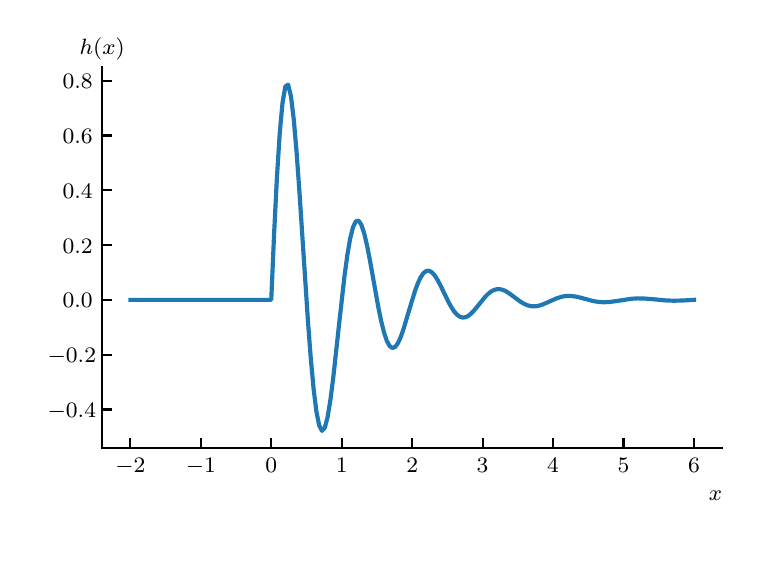
\begin{tikzpicture}%
\node[inner sep=0pt] {%% Creator: Matplotlib, PGF backend
%%
%% To include the figure in your LaTeX document, write
%%   \input{<filename>.pgf}
%%
%% Make sure the required packages are loaded in your preamble
%%   \usepackage{pgf}
%%
%% Also ensure that all the required font packages are loaded; for instance,
%% the lmodern package is sometimes necessary when using math font.
%%   \usepackage{lmodern}
%%
%% Figures using additional raster images can only be included by \input if
%% they are in the same directory as the main LaTeX file. For loading figures
%% from other directories you can use the `import` package
%%   \usepackage{import}
%%
%% and then include the figures with
%%   \import{<path to file>}{<filename>.pgf}
%%
%% Matplotlib used the following preamble
%%   \def\mathdefault#1{#1}
%%   \everymath=\expandafter{\the\everymath\displaystyle}
%%   \RequirePackage[T1]{fontenc}%
%%   \usepackage{newpxmath} % math font is Palatino compatible
%%   \let\Bbbk\relax % so it doesn't clash with amssymb
%%   \usepackage[no-math]{fontspec}
%%   \setmainfont{Palatino}
%%   \setmonofont{Latin Modern Mono}[%
%%   Scale=1.05, % a touch smaller than MatchLowercase
%%   BoldFont=*,
%%   BoldFeatures={FakeBold=2}
%%   ]
%%   \setsansfont{Helvetica}
%%   \renewcommand{\mathdefault}[1][]{}
%%   \usepackage{fontspec}
%%   \setmainfont{Palatino.ttc}[Path=\detokenize{/System/Library/Fonts/}]
%%   \setsansfont{DejaVuSans.ttf}[Path=\detokenize{/Users/ricopicone/anaconda3/envs/engcom/lib/python3.11/site-packages/matplotlib/mpl-data/fonts/ttf/}]
%%   \setmonofont{DejaVuSansMono.ttf}[Path=\detokenize{/Users/ricopicone/anaconda3/envs/engcom/lib/python3.11/site-packages/matplotlib/mpl-data/fonts/ttf/}]
%%   \makeatletter\@ifpackageloaded{underscore}{}{\usepackage[strings]{underscore}}\makeatother
%%
\begingroup%
\makeatletter%
\begin{pgfpicture}%
\pgfpathrectangle{\pgfpointorigin}{\pgfqpoint{3.572444in}{2.529415in}}%
\pgfusepath{use as bounding box, clip}%
\begin{pgfscope}%
\pgfsetbuttcap%
\pgfsetmiterjoin%
\definecolor{currentfill}{rgb}{1.000000,1.000000,1.000000}%
\pgfsetfillcolor{currentfill}%
\pgfsetlinewidth{0.000000pt}%
\definecolor{currentstroke}{rgb}{1.000000,1.000000,1.000000}%
\pgfsetstrokecolor{currentstroke}%
\pgfsetdash{}{0pt}%
\pgfpathmoveto{\pgfqpoint{0.000000in}{0.000000in}}%
\pgfpathlineto{\pgfqpoint{3.572444in}{0.000000in}}%
\pgfpathlineto{\pgfqpoint{3.572444in}{2.529415in}}%
\pgfpathlineto{\pgfqpoint{0.000000in}{2.529415in}}%
\pgfpathlineto{\pgfqpoint{0.000000in}{0.000000in}}%
\pgfpathclose%
\pgfusepath{fill}%
\end{pgfscope}%
\begin{pgfscope}%
\pgfsetbuttcap%
\pgfsetmiterjoin%
\definecolor{currentfill}{rgb}{1.000000,1.000000,1.000000}%
\pgfsetfillcolor{currentfill}%
\pgfsetlinewidth{0.000000pt}%
\definecolor{currentstroke}{rgb}{0.000000,0.000000,0.000000}%
\pgfsetstrokecolor{currentstroke}%
\pgfsetstrokeopacity{0.000000}%
\pgfsetdash{}{0pt}%
\pgfpathmoveto{\pgfqpoint{0.372444in}{0.427040in}}%
\pgfpathlineto{\pgfqpoint{3.472444in}{0.427040in}}%
\pgfpathlineto{\pgfqpoint{3.472444in}{2.330625in}}%
\pgfpathlineto{\pgfqpoint{0.372444in}{2.330625in}}%
\pgfpathlineto{\pgfqpoint{0.372444in}{0.427040in}}%
\pgfpathclose%
\pgfusepath{fill}%
\end{pgfscope}%
\begin{pgfscope}%
\pgfsetbuttcap%
\pgfsetroundjoin%
\definecolor{currentfill}{rgb}{0.000000,0.000000,0.000000}%
\pgfsetfillcolor{currentfill}%
\pgfsetlinewidth{0.803000pt}%
\definecolor{currentstroke}{rgb}{0.000000,0.000000,0.000000}%
\pgfsetstrokecolor{currentstroke}%
\pgfsetdash{}{0pt}%
\pgfsys@defobject{currentmarker}{\pgfqpoint{0.000000in}{0.000000in}}{\pgfqpoint{0.000000in}{0.048611in}}{%
\pgfpathmoveto{\pgfqpoint{0.000000in}{0.000000in}}%
\pgfpathlineto{\pgfqpoint{0.000000in}{0.048611in}}%
\pgfusepath{stroke,fill}%
}%
\begin{pgfscope}%
\pgfsys@transformshift{0.513353in}{0.427040in}%
\pgfsys@useobject{currentmarker}{}%
\end{pgfscope}%
\end{pgfscope}%
\begin{pgfscope}%
\definecolor{textcolor}{rgb}{0.000000,0.000000,0.000000}%
\pgfsetstrokecolor{textcolor}%
\pgfsetfillcolor{textcolor}%
\pgftext[x=0.513353in,y=0.378429in,,top]{\color{textcolor}{\rmfamily\fontsize{8.000000}{9.600000}\selectfont\catcode`\^=\active\def^{\ifmmode\sp\else\^{}\fi}\catcode`\%=\active\def%{\%}$\mathdefault{\ensuremath{-}2}$}}%
\end{pgfscope}%
\begin{pgfscope}%
\pgfsetbuttcap%
\pgfsetroundjoin%
\definecolor{currentfill}{rgb}{0.000000,0.000000,0.000000}%
\pgfsetfillcolor{currentfill}%
\pgfsetlinewidth{0.803000pt}%
\definecolor{currentstroke}{rgb}{0.000000,0.000000,0.000000}%
\pgfsetstrokecolor{currentstroke}%
\pgfsetdash{}{0pt}%
\pgfsys@defobject{currentmarker}{\pgfqpoint{0.000000in}{0.000000in}}{\pgfqpoint{0.000000in}{0.048611in}}{%
\pgfpathmoveto{\pgfqpoint{0.000000in}{0.000000in}}%
\pgfpathlineto{\pgfqpoint{0.000000in}{0.048611in}}%
\pgfusepath{stroke,fill}%
}%
\begin{pgfscope}%
\pgfsys@transformshift{0.865626in}{0.427040in}%
\pgfsys@useobject{currentmarker}{}%
\end{pgfscope}%
\end{pgfscope}%
\begin{pgfscope}%
\definecolor{textcolor}{rgb}{0.000000,0.000000,0.000000}%
\pgfsetstrokecolor{textcolor}%
\pgfsetfillcolor{textcolor}%
\pgftext[x=0.865626in,y=0.378429in,,top]{\color{textcolor}{\rmfamily\fontsize{8.000000}{9.600000}\selectfont\catcode`\^=\active\def^{\ifmmode\sp\else\^{}\fi}\catcode`\%=\active\def%{\%}$\mathdefault{\ensuremath{-}1}$}}%
\end{pgfscope}%
\begin{pgfscope}%
\pgfsetbuttcap%
\pgfsetroundjoin%
\definecolor{currentfill}{rgb}{0.000000,0.000000,0.000000}%
\pgfsetfillcolor{currentfill}%
\pgfsetlinewidth{0.803000pt}%
\definecolor{currentstroke}{rgb}{0.000000,0.000000,0.000000}%
\pgfsetstrokecolor{currentstroke}%
\pgfsetdash{}{0pt}%
\pgfsys@defobject{currentmarker}{\pgfqpoint{0.000000in}{0.000000in}}{\pgfqpoint{0.000000in}{0.048611in}}{%
\pgfpathmoveto{\pgfqpoint{0.000000in}{0.000000in}}%
\pgfpathlineto{\pgfqpoint{0.000000in}{0.048611in}}%
\pgfusepath{stroke,fill}%
}%
\begin{pgfscope}%
\pgfsys@transformshift{1.217899in}{0.427040in}%
\pgfsys@useobject{currentmarker}{}%
\end{pgfscope}%
\end{pgfscope}%
\begin{pgfscope}%
\definecolor{textcolor}{rgb}{0.000000,0.000000,0.000000}%
\pgfsetstrokecolor{textcolor}%
\pgfsetfillcolor{textcolor}%
\pgftext[x=1.217899in,y=0.378429in,,top]{\color{textcolor}{\rmfamily\fontsize{8.000000}{9.600000}\selectfont\catcode`\^=\active\def^{\ifmmode\sp\else\^{}\fi}\catcode`\%=\active\def%{\%}$\mathdefault{0}$}}%
\end{pgfscope}%
\begin{pgfscope}%
\pgfsetbuttcap%
\pgfsetroundjoin%
\definecolor{currentfill}{rgb}{0.000000,0.000000,0.000000}%
\pgfsetfillcolor{currentfill}%
\pgfsetlinewidth{0.803000pt}%
\definecolor{currentstroke}{rgb}{0.000000,0.000000,0.000000}%
\pgfsetstrokecolor{currentstroke}%
\pgfsetdash{}{0pt}%
\pgfsys@defobject{currentmarker}{\pgfqpoint{0.000000in}{0.000000in}}{\pgfqpoint{0.000000in}{0.048611in}}{%
\pgfpathmoveto{\pgfqpoint{0.000000in}{0.000000in}}%
\pgfpathlineto{\pgfqpoint{0.000000in}{0.048611in}}%
\pgfusepath{stroke,fill}%
}%
\begin{pgfscope}%
\pgfsys@transformshift{1.570171in}{0.427040in}%
\pgfsys@useobject{currentmarker}{}%
\end{pgfscope}%
\end{pgfscope}%
\begin{pgfscope}%
\definecolor{textcolor}{rgb}{0.000000,0.000000,0.000000}%
\pgfsetstrokecolor{textcolor}%
\pgfsetfillcolor{textcolor}%
\pgftext[x=1.570171in,y=0.378429in,,top]{\color{textcolor}{\rmfamily\fontsize{8.000000}{9.600000}\selectfont\catcode`\^=\active\def^{\ifmmode\sp\else\^{}\fi}\catcode`\%=\active\def%{\%}$\mathdefault{1}$}}%
\end{pgfscope}%
\begin{pgfscope}%
\pgfsetbuttcap%
\pgfsetroundjoin%
\definecolor{currentfill}{rgb}{0.000000,0.000000,0.000000}%
\pgfsetfillcolor{currentfill}%
\pgfsetlinewidth{0.803000pt}%
\definecolor{currentstroke}{rgb}{0.000000,0.000000,0.000000}%
\pgfsetstrokecolor{currentstroke}%
\pgfsetdash{}{0pt}%
\pgfsys@defobject{currentmarker}{\pgfqpoint{0.000000in}{0.000000in}}{\pgfqpoint{0.000000in}{0.048611in}}{%
\pgfpathmoveto{\pgfqpoint{0.000000in}{0.000000in}}%
\pgfpathlineto{\pgfqpoint{0.000000in}{0.048611in}}%
\pgfusepath{stroke,fill}%
}%
\begin{pgfscope}%
\pgfsys@transformshift{1.922444in}{0.427040in}%
\pgfsys@useobject{currentmarker}{}%
\end{pgfscope}%
\end{pgfscope}%
\begin{pgfscope}%
\definecolor{textcolor}{rgb}{0.000000,0.000000,0.000000}%
\pgfsetstrokecolor{textcolor}%
\pgfsetfillcolor{textcolor}%
\pgftext[x=1.922444in,y=0.378429in,,top]{\color{textcolor}{\rmfamily\fontsize{8.000000}{9.600000}\selectfont\catcode`\^=\active\def^{\ifmmode\sp\else\^{}\fi}\catcode`\%=\active\def%{\%}$\mathdefault{2}$}}%
\end{pgfscope}%
\begin{pgfscope}%
\pgfsetbuttcap%
\pgfsetroundjoin%
\definecolor{currentfill}{rgb}{0.000000,0.000000,0.000000}%
\pgfsetfillcolor{currentfill}%
\pgfsetlinewidth{0.803000pt}%
\definecolor{currentstroke}{rgb}{0.000000,0.000000,0.000000}%
\pgfsetstrokecolor{currentstroke}%
\pgfsetdash{}{0pt}%
\pgfsys@defobject{currentmarker}{\pgfqpoint{0.000000in}{0.000000in}}{\pgfqpoint{0.000000in}{0.048611in}}{%
\pgfpathmoveto{\pgfqpoint{0.000000in}{0.000000in}}%
\pgfpathlineto{\pgfqpoint{0.000000in}{0.048611in}}%
\pgfusepath{stroke,fill}%
}%
\begin{pgfscope}%
\pgfsys@transformshift{2.274717in}{0.427040in}%
\pgfsys@useobject{currentmarker}{}%
\end{pgfscope}%
\end{pgfscope}%
\begin{pgfscope}%
\definecolor{textcolor}{rgb}{0.000000,0.000000,0.000000}%
\pgfsetstrokecolor{textcolor}%
\pgfsetfillcolor{textcolor}%
\pgftext[x=2.274717in,y=0.378429in,,top]{\color{textcolor}{\rmfamily\fontsize{8.000000}{9.600000}\selectfont\catcode`\^=\active\def^{\ifmmode\sp\else\^{}\fi}\catcode`\%=\active\def%{\%}$\mathdefault{3}$}}%
\end{pgfscope}%
\begin{pgfscope}%
\pgfsetbuttcap%
\pgfsetroundjoin%
\definecolor{currentfill}{rgb}{0.000000,0.000000,0.000000}%
\pgfsetfillcolor{currentfill}%
\pgfsetlinewidth{0.803000pt}%
\definecolor{currentstroke}{rgb}{0.000000,0.000000,0.000000}%
\pgfsetstrokecolor{currentstroke}%
\pgfsetdash{}{0pt}%
\pgfsys@defobject{currentmarker}{\pgfqpoint{0.000000in}{0.000000in}}{\pgfqpoint{0.000000in}{0.048611in}}{%
\pgfpathmoveto{\pgfqpoint{0.000000in}{0.000000in}}%
\pgfpathlineto{\pgfqpoint{0.000000in}{0.048611in}}%
\pgfusepath{stroke,fill}%
}%
\begin{pgfscope}%
\pgfsys@transformshift{2.626990in}{0.427040in}%
\pgfsys@useobject{currentmarker}{}%
\end{pgfscope}%
\end{pgfscope}%
\begin{pgfscope}%
\definecolor{textcolor}{rgb}{0.000000,0.000000,0.000000}%
\pgfsetstrokecolor{textcolor}%
\pgfsetfillcolor{textcolor}%
\pgftext[x=2.626990in,y=0.378429in,,top]{\color{textcolor}{\rmfamily\fontsize{8.000000}{9.600000}\selectfont\catcode`\^=\active\def^{\ifmmode\sp\else\^{}\fi}\catcode`\%=\active\def%{\%}$\mathdefault{4}$}}%
\end{pgfscope}%
\begin{pgfscope}%
\pgfsetbuttcap%
\pgfsetroundjoin%
\definecolor{currentfill}{rgb}{0.000000,0.000000,0.000000}%
\pgfsetfillcolor{currentfill}%
\pgfsetlinewidth{0.803000pt}%
\definecolor{currentstroke}{rgb}{0.000000,0.000000,0.000000}%
\pgfsetstrokecolor{currentstroke}%
\pgfsetdash{}{0pt}%
\pgfsys@defobject{currentmarker}{\pgfqpoint{0.000000in}{0.000000in}}{\pgfqpoint{0.000000in}{0.048611in}}{%
\pgfpathmoveto{\pgfqpoint{0.000000in}{0.000000in}}%
\pgfpathlineto{\pgfqpoint{0.000000in}{0.048611in}}%
\pgfusepath{stroke,fill}%
}%
\begin{pgfscope}%
\pgfsys@transformshift{2.979262in}{0.427040in}%
\pgfsys@useobject{currentmarker}{}%
\end{pgfscope}%
\end{pgfscope}%
\begin{pgfscope}%
\definecolor{textcolor}{rgb}{0.000000,0.000000,0.000000}%
\pgfsetstrokecolor{textcolor}%
\pgfsetfillcolor{textcolor}%
\pgftext[x=2.979262in,y=0.378429in,,top]{\color{textcolor}{\rmfamily\fontsize{8.000000}{9.600000}\selectfont\catcode`\^=\active\def^{\ifmmode\sp\else\^{}\fi}\catcode`\%=\active\def%{\%}$\mathdefault{5}$}}%
\end{pgfscope}%
\begin{pgfscope}%
\pgfsetbuttcap%
\pgfsetroundjoin%
\definecolor{currentfill}{rgb}{0.000000,0.000000,0.000000}%
\pgfsetfillcolor{currentfill}%
\pgfsetlinewidth{0.803000pt}%
\definecolor{currentstroke}{rgb}{0.000000,0.000000,0.000000}%
\pgfsetstrokecolor{currentstroke}%
\pgfsetdash{}{0pt}%
\pgfsys@defobject{currentmarker}{\pgfqpoint{0.000000in}{0.000000in}}{\pgfqpoint{0.000000in}{0.048611in}}{%
\pgfpathmoveto{\pgfqpoint{0.000000in}{0.000000in}}%
\pgfpathlineto{\pgfqpoint{0.000000in}{0.048611in}}%
\pgfusepath{stroke,fill}%
}%
\begin{pgfscope}%
\pgfsys@transformshift{3.331535in}{0.427040in}%
\pgfsys@useobject{currentmarker}{}%
\end{pgfscope}%
\end{pgfscope}%
\begin{pgfscope}%
\definecolor{textcolor}{rgb}{0.000000,0.000000,0.000000}%
\pgfsetstrokecolor{textcolor}%
\pgfsetfillcolor{textcolor}%
\pgftext[x=3.331535in,y=0.378429in,,top]{\color{textcolor}{\rmfamily\fontsize{8.000000}{9.600000}\selectfont\catcode`\^=\active\def^{\ifmmode\sp\else\^{}\fi}\catcode`\%=\active\def%{\%}$\mathdefault{6}$}}%
\end{pgfscope}%
\begin{pgfscope}%
\definecolor{textcolor}{rgb}{0.000000,0.000000,0.000000}%
\pgfsetstrokecolor{textcolor}%
\pgfsetfillcolor{textcolor}%
\pgftext[x=3.472444in,y=0.211437in,right,top]{\color{textcolor}{\rmfamily\fontsize{8.000000}{9.600000}\selectfont\catcode`\^=\active\def^{\ifmmode\sp\else\^{}\fi}\catcode`\%=\active\def%{\%}$x$}}%
\end{pgfscope}%
\begin{pgfscope}%
\pgfsetbuttcap%
\pgfsetroundjoin%
\definecolor{currentfill}{rgb}{0.000000,0.000000,0.000000}%
\pgfsetfillcolor{currentfill}%
\pgfsetlinewidth{0.803000pt}%
\definecolor{currentstroke}{rgb}{0.000000,0.000000,0.000000}%
\pgfsetstrokecolor{currentstroke}%
\pgfsetdash{}{0pt}%
\pgfsys@defobject{currentmarker}{\pgfqpoint{0.000000in}{0.000000in}}{\pgfqpoint{0.048611in}{0.000000in}}{%
\pgfpathmoveto{\pgfqpoint{0.000000in}{0.000000in}}%
\pgfpathlineto{\pgfqpoint{0.048611in}{0.000000in}}%
\pgfusepath{stroke,fill}%
}%
\begin{pgfscope}%
\pgfsys@transformshift{0.372444in}{0.620602in}%
\pgfsys@useobject{currentmarker}{}%
\end{pgfscope}%
\end{pgfscope}%
\begin{pgfscope}%
\definecolor{textcolor}{rgb}{0.000000,0.000000,0.000000}%
\pgfsetstrokecolor{textcolor}%
\pgfsetfillcolor{textcolor}%
\pgftext[x=0.100000in, y=0.580183in, left, base]{\color{textcolor}{\rmfamily\fontsize{8.000000}{9.600000}\selectfont\catcode`\^=\active\def^{\ifmmode\sp\else\^{}\fi}\catcode`\%=\active\def%{\%}$\mathdefault{\ensuremath{-}0.4}$}}%
\end{pgfscope}%
\begin{pgfscope}%
\pgfsetbuttcap%
\pgfsetroundjoin%
\definecolor{currentfill}{rgb}{0.000000,0.000000,0.000000}%
\pgfsetfillcolor{currentfill}%
\pgfsetlinewidth{0.803000pt}%
\definecolor{currentstroke}{rgb}{0.000000,0.000000,0.000000}%
\pgfsetstrokecolor{currentstroke}%
\pgfsetdash{}{0pt}%
\pgfsys@defobject{currentmarker}{\pgfqpoint{0.000000in}{0.000000in}}{\pgfqpoint{0.048611in}{0.000000in}}{%
\pgfpathmoveto{\pgfqpoint{0.000000in}{0.000000in}}%
\pgfpathlineto{\pgfqpoint{0.048611in}{0.000000in}}%
\pgfusepath{stroke,fill}%
}%
\begin{pgfscope}%
\pgfsys@transformshift{0.372444in}{0.894592in}%
\pgfsys@useobject{currentmarker}{}%
\end{pgfscope}%
\end{pgfscope}%
\begin{pgfscope}%
\definecolor{textcolor}{rgb}{0.000000,0.000000,0.000000}%
\pgfsetstrokecolor{textcolor}%
\pgfsetfillcolor{textcolor}%
\pgftext[x=0.100000in, y=0.854173in, left, base]{\color{textcolor}{\rmfamily\fontsize{8.000000}{9.600000}\selectfont\catcode`\^=\active\def^{\ifmmode\sp\else\^{}\fi}\catcode`\%=\active\def%{\%}$\mathdefault{\ensuremath{-}0.2}$}}%
\end{pgfscope}%
\begin{pgfscope}%
\pgfsetbuttcap%
\pgfsetroundjoin%
\definecolor{currentfill}{rgb}{0.000000,0.000000,0.000000}%
\pgfsetfillcolor{currentfill}%
\pgfsetlinewidth{0.803000pt}%
\definecolor{currentstroke}{rgb}{0.000000,0.000000,0.000000}%
\pgfsetstrokecolor{currentstroke}%
\pgfsetdash{}{0pt}%
\pgfsys@defobject{currentmarker}{\pgfqpoint{0.000000in}{0.000000in}}{\pgfqpoint{0.048611in}{0.000000in}}{%
\pgfpathmoveto{\pgfqpoint{0.000000in}{0.000000in}}%
\pgfpathlineto{\pgfqpoint{0.048611in}{0.000000in}}%
\pgfusepath{stroke,fill}%
}%
\begin{pgfscope}%
\pgfsys@transformshift{0.372444in}{1.168582in}%
\pgfsys@useobject{currentmarker}{}%
\end{pgfscope}%
\end{pgfscope}%
\begin{pgfscope}%
\definecolor{textcolor}{rgb}{0.000000,0.000000,0.000000}%
\pgfsetstrokecolor{textcolor}%
\pgfsetfillcolor{textcolor}%
\pgftext[x=0.174333in, y=1.128164in, left, base]{\color{textcolor}{\rmfamily\fontsize{8.000000}{9.600000}\selectfont\catcode`\^=\active\def^{\ifmmode\sp\else\^{}\fi}\catcode`\%=\active\def%{\%}$\mathdefault{0.0}$}}%
\end{pgfscope}%
\begin{pgfscope}%
\pgfsetbuttcap%
\pgfsetroundjoin%
\definecolor{currentfill}{rgb}{0.000000,0.000000,0.000000}%
\pgfsetfillcolor{currentfill}%
\pgfsetlinewidth{0.803000pt}%
\definecolor{currentstroke}{rgb}{0.000000,0.000000,0.000000}%
\pgfsetstrokecolor{currentstroke}%
\pgfsetdash{}{0pt}%
\pgfsys@defobject{currentmarker}{\pgfqpoint{0.000000in}{0.000000in}}{\pgfqpoint{0.048611in}{0.000000in}}{%
\pgfpathmoveto{\pgfqpoint{0.000000in}{0.000000in}}%
\pgfpathlineto{\pgfqpoint{0.048611in}{0.000000in}}%
\pgfusepath{stroke,fill}%
}%
\begin{pgfscope}%
\pgfsys@transformshift{0.372444in}{1.442573in}%
\pgfsys@useobject{currentmarker}{}%
\end{pgfscope}%
\end{pgfscope}%
\begin{pgfscope}%
\definecolor{textcolor}{rgb}{0.000000,0.000000,0.000000}%
\pgfsetstrokecolor{textcolor}%
\pgfsetfillcolor{textcolor}%
\pgftext[x=0.174333in, y=1.402154in, left, base]{\color{textcolor}{\rmfamily\fontsize{8.000000}{9.600000}\selectfont\catcode`\^=\active\def^{\ifmmode\sp\else\^{}\fi}\catcode`\%=\active\def%{\%}$\mathdefault{0.2}$}}%
\end{pgfscope}%
\begin{pgfscope}%
\pgfsetbuttcap%
\pgfsetroundjoin%
\definecolor{currentfill}{rgb}{0.000000,0.000000,0.000000}%
\pgfsetfillcolor{currentfill}%
\pgfsetlinewidth{0.803000pt}%
\definecolor{currentstroke}{rgb}{0.000000,0.000000,0.000000}%
\pgfsetstrokecolor{currentstroke}%
\pgfsetdash{}{0pt}%
\pgfsys@defobject{currentmarker}{\pgfqpoint{0.000000in}{0.000000in}}{\pgfqpoint{0.048611in}{0.000000in}}{%
\pgfpathmoveto{\pgfqpoint{0.000000in}{0.000000in}}%
\pgfpathlineto{\pgfqpoint{0.048611in}{0.000000in}}%
\pgfusepath{stroke,fill}%
}%
\begin{pgfscope}%
\pgfsys@transformshift{0.372444in}{1.716563in}%
\pgfsys@useobject{currentmarker}{}%
\end{pgfscope}%
\end{pgfscope}%
\begin{pgfscope}%
\definecolor{textcolor}{rgb}{0.000000,0.000000,0.000000}%
\pgfsetstrokecolor{textcolor}%
\pgfsetfillcolor{textcolor}%
\pgftext[x=0.174333in, y=1.676144in, left, base]{\color{textcolor}{\rmfamily\fontsize{8.000000}{9.600000}\selectfont\catcode`\^=\active\def^{\ifmmode\sp\else\^{}\fi}\catcode`\%=\active\def%{\%}$\mathdefault{0.4}$}}%
\end{pgfscope}%
\begin{pgfscope}%
\pgfsetbuttcap%
\pgfsetroundjoin%
\definecolor{currentfill}{rgb}{0.000000,0.000000,0.000000}%
\pgfsetfillcolor{currentfill}%
\pgfsetlinewidth{0.803000pt}%
\definecolor{currentstroke}{rgb}{0.000000,0.000000,0.000000}%
\pgfsetstrokecolor{currentstroke}%
\pgfsetdash{}{0pt}%
\pgfsys@defobject{currentmarker}{\pgfqpoint{0.000000in}{0.000000in}}{\pgfqpoint{0.048611in}{0.000000in}}{%
\pgfpathmoveto{\pgfqpoint{0.000000in}{0.000000in}}%
\pgfpathlineto{\pgfqpoint{0.048611in}{0.000000in}}%
\pgfusepath{stroke,fill}%
}%
\begin{pgfscope}%
\pgfsys@transformshift{0.372444in}{1.990553in}%
\pgfsys@useobject{currentmarker}{}%
\end{pgfscope}%
\end{pgfscope}%
\begin{pgfscope}%
\definecolor{textcolor}{rgb}{0.000000,0.000000,0.000000}%
\pgfsetstrokecolor{textcolor}%
\pgfsetfillcolor{textcolor}%
\pgftext[x=0.174333in, y=1.950135in, left, base]{\color{textcolor}{\rmfamily\fontsize{8.000000}{9.600000}\selectfont\catcode`\^=\active\def^{\ifmmode\sp\else\^{}\fi}\catcode`\%=\active\def%{\%}$\mathdefault{0.6}$}}%
\end{pgfscope}%
\begin{pgfscope}%
\pgfsetbuttcap%
\pgfsetroundjoin%
\definecolor{currentfill}{rgb}{0.000000,0.000000,0.000000}%
\pgfsetfillcolor{currentfill}%
\pgfsetlinewidth{0.803000pt}%
\definecolor{currentstroke}{rgb}{0.000000,0.000000,0.000000}%
\pgfsetstrokecolor{currentstroke}%
\pgfsetdash{}{0pt}%
\pgfsys@defobject{currentmarker}{\pgfqpoint{0.000000in}{0.000000in}}{\pgfqpoint{0.048611in}{0.000000in}}{%
\pgfpathmoveto{\pgfqpoint{0.000000in}{0.000000in}}%
\pgfpathlineto{\pgfqpoint{0.048611in}{0.000000in}}%
\pgfusepath{stroke,fill}%
}%
\begin{pgfscope}%
\pgfsys@transformshift{0.372444in}{2.264544in}%
\pgfsys@useobject{currentmarker}{}%
\end{pgfscope}%
\end{pgfscope}%
\begin{pgfscope}%
\definecolor{textcolor}{rgb}{0.000000,0.000000,0.000000}%
\pgfsetstrokecolor{textcolor}%
\pgfsetfillcolor{textcolor}%
\pgftext[x=0.174333in, y=2.224125in, left, base]{\color{textcolor}{\rmfamily\fontsize{8.000000}{9.600000}\selectfont\catcode`\^=\active\def^{\ifmmode\sp\else\^{}\fi}\catcode`\%=\active\def%{\%}$\mathdefault{0.8}$}}%
\end{pgfscope}%
\begin{pgfscope}%
\definecolor{textcolor}{rgb}{0.000000,0.000000,0.000000}%
\pgfsetstrokecolor{textcolor}%
\pgfsetfillcolor{textcolor}%
\pgftext[x=0.372444in,y=2.368696in,,bottom]{\color{textcolor}{\rmfamily\fontsize{8.000000}{9.600000}\selectfont\catcode`\^=\active\def^{\ifmmode\sp\else\^{}\fi}\catcode`\%=\active\def%{\%}$h(x)$}}%
\end{pgfscope}%
\begin{pgfscope}%
\pgfpathrectangle{\pgfqpoint{0.372444in}{0.427040in}}{\pgfqpoint{3.100000in}{1.903585in}}%
\pgfusepath{clip}%
\pgfsetrectcap%
\pgfsetroundjoin%
\pgfsetlinewidth{1.505625pt}%
\definecolor{currentstroke}{rgb}{0.121569,0.466667,0.705882}%
\pgfsetstrokecolor{currentstroke}%
\pgfsetdash{}{0pt}%
\pgfpathmoveto{\pgfqpoint{0.513353in}{1.168582in}}%
\pgfpathlineto{\pgfqpoint{1.217899in}{1.168582in}}%
\pgfpathlineto{\pgfqpoint{1.231990in}{1.495917in}}%
\pgfpathlineto{\pgfqpoint{1.246081in}{1.777820in}}%
\pgfpathlineto{\pgfqpoint{1.260171in}{2.000333in}}%
\pgfpathlineto{\pgfqpoint{1.274262in}{2.154247in}}%
\pgfpathlineto{\pgfqpoint{1.288353in}{2.235308in}}%
\pgfpathlineto{\pgfqpoint{1.302444in}{2.244098in}}%
\pgfpathlineto{\pgfqpoint{1.316535in}{2.185630in}}%
\pgfpathlineto{\pgfqpoint{1.330626in}{2.068694in}}%
\pgfpathlineto{\pgfqpoint{1.344717in}{1.905026in}}%
\pgfpathlineto{\pgfqpoint{1.358808in}{1.708349in}}%
\pgfpathlineto{\pgfqpoint{1.401081in}{1.066503in}}%
\pgfpathlineto{\pgfqpoint{1.415171in}{0.880514in}}%
\pgfpathlineto{\pgfqpoint{1.429262in}{0.726659in}}%
\pgfpathlineto{\pgfqpoint{1.443353in}{0.611990in}}%
\pgfpathlineto{\pgfqpoint{1.457444in}{0.540595in}}%
\pgfpathlineto{\pgfqpoint{1.471535in}{0.513567in}}%
\pgfpathlineto{\pgfqpoint{1.485626in}{0.529166in}}%
\pgfpathlineto{\pgfqpoint{1.499717in}{0.583151in}}%
\pgfpathlineto{\pgfqpoint{1.513808in}{0.669228in}}%
\pgfpathlineto{\pgfqpoint{1.527899in}{0.779600in}}%
\pgfpathlineto{\pgfqpoint{1.556081in}{1.038133in}}%
\pgfpathlineto{\pgfqpoint{1.584262in}{1.289002in}}%
\pgfpathlineto{\pgfqpoint{1.598353in}{1.392708in}}%
\pgfpathlineto{\pgfqpoint{1.612444in}{1.474566in}}%
\pgfpathlineto{\pgfqpoint{1.626535in}{1.531188in}}%
\pgfpathlineto{\pgfqpoint{1.640626in}{1.561009in}}%
\pgfpathlineto{\pgfqpoint{1.654717in}{1.564242in}}%
\pgfpathlineto{\pgfqpoint{1.668808in}{1.542733in}}%
\pgfpathlineto{\pgfqpoint{1.682899in}{1.499715in}}%
\pgfpathlineto{\pgfqpoint{1.696990in}{1.439505in}}%
\pgfpathlineto{\pgfqpoint{1.711081in}{1.367151in}}%
\pgfpathlineto{\pgfqpoint{1.753353in}{1.131029in}}%
\pgfpathlineto{\pgfqpoint{1.767444in}{1.062608in}}%
\pgfpathlineto{\pgfqpoint{1.781535in}{1.006008in}}%
\pgfpathlineto{\pgfqpoint{1.795626in}{0.963824in}}%
\pgfpathlineto{\pgfqpoint{1.809717in}{0.937559in}}%
\pgfpathlineto{\pgfqpoint{1.823808in}{0.927616in}}%
\pgfpathlineto{\pgfqpoint{1.837899in}{0.933354in}}%
\pgfpathlineto{\pgfqpoint{1.851990in}{0.953214in}}%
\pgfpathlineto{\pgfqpoint{1.866081in}{0.984880in}}%
\pgfpathlineto{\pgfqpoint{1.880171in}{1.025484in}}%
\pgfpathlineto{\pgfqpoint{1.908353in}{1.120593in}}%
\pgfpathlineto{\pgfqpoint{1.936535in}{1.212882in}}%
\pgfpathlineto{\pgfqpoint{1.950626in}{1.251034in}}%
\pgfpathlineto{\pgfqpoint{1.964717in}{1.281148in}}%
\pgfpathlineto{\pgfqpoint{1.978808in}{1.301978in}}%
\pgfpathlineto{\pgfqpoint{1.992899in}{1.312948in}}%
\pgfpathlineto{\pgfqpoint{2.006990in}{1.314138in}}%
\pgfpathlineto{\pgfqpoint{2.021081in}{1.306225in}}%
\pgfpathlineto{\pgfqpoint{2.035171in}{1.290399in}}%
\pgfpathlineto{\pgfqpoint{2.049262in}{1.268249in}}%
\pgfpathlineto{\pgfqpoint{2.063353in}{1.241632in}}%
\pgfpathlineto{\pgfqpoint{2.105626in}{1.154767in}}%
\pgfpathlineto{\pgfqpoint{2.119717in}{1.129597in}}%
\pgfpathlineto{\pgfqpoint{2.133808in}{1.108774in}}%
\pgfpathlineto{\pgfqpoint{2.147899in}{1.093256in}}%
\pgfpathlineto{\pgfqpoint{2.161990in}{1.083594in}}%
\pgfpathlineto{\pgfqpoint{2.176081in}{1.079936in}}%
\pgfpathlineto{\pgfqpoint{2.190171in}{1.082047in}}%
\pgfpathlineto{\pgfqpoint{2.204262in}{1.089353in}}%
\pgfpathlineto{\pgfqpoint{2.218353in}{1.101002in}}%
\pgfpathlineto{\pgfqpoint{2.232444in}{1.115939in}}%
\pgfpathlineto{\pgfqpoint{2.288808in}{1.184879in}}%
\pgfpathlineto{\pgfqpoint{2.302899in}{1.198915in}}%
\pgfpathlineto{\pgfqpoint{2.316990in}{1.209993in}}%
\pgfpathlineto{\pgfqpoint{2.331081in}{1.217656in}}%
\pgfpathlineto{\pgfqpoint{2.345171in}{1.221691in}}%
\pgfpathlineto{\pgfqpoint{2.359262in}{1.222129in}}%
\pgfpathlineto{\pgfqpoint{2.373353in}{1.219218in}}%
\pgfpathlineto{\pgfqpoint{2.387444in}{1.213396in}}%
\pgfpathlineto{\pgfqpoint{2.401535in}{1.205248in}}%
\pgfpathlineto{\pgfqpoint{2.429717in}{1.184753in}}%
\pgfpathlineto{\pgfqpoint{2.457899in}{1.163500in}}%
\pgfpathlineto{\pgfqpoint{2.471990in}{1.154240in}}%
\pgfpathlineto{\pgfqpoint{2.486081in}{1.146580in}}%
\pgfpathlineto{\pgfqpoint{2.500171in}{1.140871in}}%
\pgfpathlineto{\pgfqpoint{2.514262in}{1.137317in}}%
\pgfpathlineto{\pgfqpoint{2.528353in}{1.135971in}}%
\pgfpathlineto{\pgfqpoint{2.542444in}{1.136748in}}%
\pgfpathlineto{\pgfqpoint{2.556535in}{1.139435in}}%
\pgfpathlineto{\pgfqpoint{2.570626in}{1.143721in}}%
\pgfpathlineto{\pgfqpoint{2.598808in}{1.155488in}}%
\pgfpathlineto{\pgfqpoint{2.641081in}{1.174578in}}%
\pgfpathlineto{\pgfqpoint{2.669262in}{1.183816in}}%
\pgfpathlineto{\pgfqpoint{2.683353in}{1.186635in}}%
\pgfpathlineto{\pgfqpoint{2.697444in}{1.188120in}}%
\pgfpathlineto{\pgfqpoint{2.711535in}{1.188281in}}%
\pgfpathlineto{\pgfqpoint{2.739717in}{1.185068in}}%
\pgfpathlineto{\pgfqpoint{2.767899in}{1.178469in}}%
\pgfpathlineto{\pgfqpoint{2.824262in}{1.163306in}}%
\pgfpathlineto{\pgfqpoint{2.852444in}{1.158388in}}%
\pgfpathlineto{\pgfqpoint{2.880626in}{1.156585in}}%
\pgfpathlineto{\pgfqpoint{2.908808in}{1.157860in}}%
\pgfpathlineto{\pgfqpoint{2.936990in}{1.161458in}}%
\pgfpathlineto{\pgfqpoint{3.021535in}{1.174187in}}%
\pgfpathlineto{\pgfqpoint{3.049717in}{1.175770in}}%
\pgfpathlineto{\pgfqpoint{3.077899in}{1.175435in}}%
\pgfpathlineto{\pgfqpoint{3.120171in}{1.172219in}}%
\pgfpathlineto{\pgfqpoint{3.190626in}{1.165605in}}%
\pgfpathlineto{\pgfqpoint{3.232899in}{1.164169in}}%
\pgfpathlineto{\pgfqpoint{3.275171in}{1.165218in}}%
\pgfpathlineto{\pgfqpoint{3.331535in}{1.168582in}}%
\pgfpathlineto{\pgfqpoint{3.331535in}{1.168582in}}%
\pgfusepath{stroke}%
\end{pgfscope}%
\begin{pgfscope}%
\pgfsetrectcap%
\pgfsetmiterjoin%
\pgfsetlinewidth{0.803000pt}%
\definecolor{currentstroke}{rgb}{0.000000,0.000000,0.000000}%
\pgfsetstrokecolor{currentstroke}%
\pgfsetdash{}{0pt}%
\pgfpathmoveto{\pgfqpoint{0.372444in}{0.427040in}}%
\pgfpathlineto{\pgfqpoint{0.372444in}{2.330625in}}%
\pgfusepath{stroke}%
\end{pgfscope}%
\begin{pgfscope}%
\pgfsetrectcap%
\pgfsetmiterjoin%
\pgfsetlinewidth{0.803000pt}%
\definecolor{currentstroke}{rgb}{0.000000,0.000000,0.000000}%
\pgfsetstrokecolor{currentstroke}%
\pgfsetdash{}{0pt}%
\pgfpathmoveto{\pgfqpoint{0.372444in}{0.427040in}}%
\pgfpathlineto{\pgfqpoint{3.472444in}{0.427040in}}%
\pgfusepath{stroke}%
\end{pgfscope}%
\end{pgfpicture}%
\makeatother%
\endgroup%
};%
\end{tikzpicture}%
\caption{}
\label{fig:publishing_with_makefile-figure-2}
\end{figure}

\phantomsection\label{fa09f205}
\nointerlineskip\nointerlineskip\begin{minted}[autogobble,samepage]{python}
plt.show()
\end{minted}
